%File: anonymous-submission-latex-2024.tex
\documentclass[letterpaper]{article} % DO NOT CHANGE THIS
\usepackage{aaai24}  % DO NOT CHANGE THIS
\usepackage{times}  % DO NOT CHANGE THIS
\usepackage{helvet}  % DO NOT CHANGE THIS
\usepackage{courier}  % DO NOT CHANGE THIS
\usepackage[hyphens]{url}  % DO NOT CHANGE THIS
\usepackage{graphicx} % DO NOT CHANGE THIS
\urlstyle{rm} % DO NOT CHANGE THIS
\def\UrlFont{\rm}  % DO NOT CHANGE THIS
\usepackage{natbib}  % DO NOT CHANGE THIS AND DO NOT ADD ANY OPTIONS TO IT
\usepackage{caption} % DO NOT CHANGE THIS AND DO NOT ADD ANY OPTIONS TO IT
\frenchspacing  % DO NOT CHANGE THIS
\setlength{\pdfpagewidth}{8.5in} % DO NOT CHANGE THIS
\setlength{\pdfpageheight}{11in} % DO NOT CHANGE THIS
%
% These are recommended to typeset algorithms but not required. See the subsubsection on algorithms. Remove them if you don't have algorithms in your paper.
\usepackage{algorithm}
\usepackage{algorithmic}
\usepackage{multirow}
% \usepackage{bbm}
\usepackage{amsmath,amscd,amsbsy,amssymb,latexsym,url,bm,amsthm}

\newtheorem{remark}{Remark}
\newtheorem{corollary}{Corollary}
\newtheorem{theorem}{Theorem}
\newtheorem{assumption}{Assumption}
\newtheorem{lemma}{Lemma}
\newtheorem{claim}{Claim}
\newtheorem{fact}{Fact}
\newtheorem{definition}{Definition}
\newtheorem{example}{Example}



\usepackage[utf8]{inputenc} % allow utf-8 input
\usepackage[T1]{fontenc}    % use 8-bit T1 fonts
% \usepackage{hyperref}       % hyperlinks
\usepackage{url}            % simple URL typesetting
\usepackage{booktabs}       % professional-quality tables
\usepackage{amsfonts}       % blackboard math symbols
\usepackage{nicefrac}       % compact symbols for 1/2, etc.
\usepackage{microtype}      % microtypography
\usepackage{algorithm,algorithmic}
% \usepackage{xcolor}         % colors

\usepackage{amsmath,amscd,amsbsy,amssymb,latexsym,url,bm,amsthm}
\allowdisplaybreaks
\usepackage{cleveref}
\usepackage{verbatim}
\usepackage{color}
\usepackage{dsfont}
% \newtheorem{remark}{Remark}
% \newtheorem{corollary}{Corollary}
% \newtheorem{theorem}{Theorem}
% \newtheorem{assumption}{Assumption}
% \newtheorem{lemma}{Lemma}
% \newtheorem{claim}{Claim}
% \newtheorem{fact}{Fact}
% \newtheorem{definition}{Definition}
% \newtheorem{example}{Example}

\newcommand{\set}[1]{\left\{ #1 \right\}}
\newcommand{\NN}{\mathbb{N}}
\newcommand{\RR}{\mathbb{R}}
\newcommand{\cA}{\mathcal{A}}
\newcommand{\cB}{\mathcal{B}}
\newcommand{\cC}{\mathcal{C}}
\newcommand{\cE}{\mathcal{E}}
\newcommand{\cF}{\mathcal{F}}
\newcommand{\cH}{\mathcal{H}}
\newcommand{\cI}{\mathcal{I}}
\newcommand{\cS}{\mathcal{S}}
\newcommand{\cN}{\mathcal{N}}
\newcommand{\cU}{\mathcal{U}}
\newcommand{\cK}{\mathcal{K}}
\newcommand{\Beta}{\mathrm{Beta}}
\newcommand{\true}{\mathrm{True}}
\newcommand{\false}{\mathrm{False}}
\newcommand{\flag}{{\mathrm{F}}}
\newcommand{\ucb}{{\mathrm{UCB}}}
\newcommand{\lcb}{{\mathrm{LCB}}}
\newcommand{\opt}{{\mathrm{opt}}}

\newcommand{\trace}{\mathrm{trace}}
\newcommand{\abs}[1]{\left| #1 \right|}
\newcommand{\bOne}[1]{\mathds{1} \! \left\{#1\right\}}
\newcommand{\bracket}[1]{\left(#1\right)}
\newcommand{\norm}[1]{\left\| #1 \right\|}

\newcommand{\EE}[1]{\mathbb{E} \left[#1\right]}
\newcommand{\PP}[1]{\mathbb{P} \left(#1\right)}
\newcommand{\pluseq}{\mathrel{+}=}
\newcommand{\etal}{\emph{et al.}}



\usepackage{tikz}
\usetikzlibrary{shapes,shapes.misc,positioning}
\usetikzlibrary{patterns,arrows,decorations.pathreplacing}
\newcommand{\tikzmarkC}[1]{\tikz[overlay,remember picture,baseline={-3pt}] \node[] (#1) {};}


\DeclareMathOperator*{\argmax}{argmax}
\DeclareMathOperator*{\argmin}{argmin}


\mathchardef\mhyphen="2D
\newcommand{\ch}{{\tt Ch}}









%
% These are are recommended to typeset listings but not required. See the subsubsection on listing. Remove this block if you don't have listings in your paper.
\usepackage{newfloat}
\usepackage{listings}
\DeclareCaptionStyle{ruled}{labelfont=normalfont,labelsep=colon,strut=off} % DO NOT CHANGE THIS
\lstset{%
	basicstyle={\footnotesize\ttfamily},% footnotesize acceptable for monospace
	numbers=left,numberstyle=\footnotesize,xleftmargin=2em,% show line numbers, remove this entire line if you don't want the numbers.
	aboveskip=0pt,belowskip=0pt,%
	showstringspaces=false,tabsize=2,breaklines=true}
\floatstyle{ruled}
\newfloat{listing}{tb}{lst}{}
\floatname{listing}{Listing}
%
% Keep the \pdfinfo as shown here. There's no need
% for you to add the /Title and /Author tags.

% DISALLOWED PACKAGES
% \usepackage{authblk} -- This package is specifically forbidden
% \usepackage{balance} -- This package is specifically forbidden
% \usepackage{color (if used in text)
% \usepackage{CJK} -- This package is specifically forbidden
% \usepackage{float} -- This package is specifically forbidden
% \usepackage{flushend} -- This package is specifically forbidden
% \usepackage{fontenc} -- This package is specifically forbidden
% \usepackage{fullpage} -- This package is specifically forbidden
% \usepackage{geometry} -- This package is specifically forbidden
% \usepackage{grffile} -- This package is specifically forbidden
% \usepackage{hyperref} -- This package is specifically forbidden
% \usepackage{navigator} -- This package is specifically forbidden
% (or any other package that embeds links such as navigator or hyperref)
% \indentfirst} -- This package is specifically forbidden
% \layout} -- This package is specifically forbidden
% \multicol} -- This package is specifically forbidden
% \nameref} -- This package is specifically forbidden
% \usepackage{savetrees} -- This package is specifically forbidden
% \usepackage{setspace} -- This package is specifically forbidden
% \usepackage{stfloats} -- This package is specifically forbidden
% \usepackage{tabu} -- This package is specifically forbidden
% \usepackage{titlesec} -- This package is specifically forbidden
% \usepackage{tocbibind} -- This package is specifically forbidden
% \usepackage{ulem} -- This package is specifically forbidden
% \usepackage{wrapfig} -- This package is specifically forbidden
% DISALLOWED COMMANDS
% \nocopyright -- Your paper will not be published if you use this command
% \addtolength -- This command may not be used
% \balance -- This command may not be used
% \baselinestretch -- Your paper will not be published if you use this command
% \clearpage -- No page breaks of any kind may be used for the final version of your paper
% \columnsep -- This command may not be used
% % \newpage -- No page breaks of any kind may be used for the final version of your paper
% \pagebreak -- No page breaks of any kind may be used for the final version of your paperr
% \pagestyle -- This command may not be used
% \tiny -- This is not an acceptable font size.
% \vspace{- -- No negative value may be used in proximity of a caption, figure, table, section, subsection, subsubsection, or reference
% \vskip{- -- No negative value may be used to alter spacing above or below a caption, figure, table, section, subsection, subsubsection, or reference

\setcounter{secnumdepth}{2} %May be changed to 1 or 2 if section numbers are desired.

% The file aaai24.sty is the style file for AAAI Press
% proceedings, working notes, and technical reports.
%

% Title

% Your title must be in mixed case, not sentence case.
% That means all verbs (including short verbs like be, is, using,and go),
% nouns, adverbs, adjectives should be capitalized, including both words in hyphenated terms, while
% articles, conjunctions, and prepositions are lower case unless they
% directly follow a colon or long dash
\title{
% Regret Bounds for
Improved Bandits in Many-to-one Matching Markets with Incentive Compatibility
}

\author {
    % Authors
    Fang Kong, Shuai Li\thanks{Corresponding author.}
}
\affiliations {
    % Affiliations
    % \textsuperscript{\rm 1}
    John Hopcroft Center for Computer Science, Shanghai Jiao Tong University \\
    % \textsuperscript{\rm 2}Affiliation 2\\
    \{fangkong, shuaili8\}@sjtu.edu.cn
    % , secondAuthor@affilation2.com, thirdAuthor@affiliation1.com
}



% \author{
%     %Authors
%     % All authors must be in the same font size and format.
%     Written by AAAI Press Staff\textsuperscript{\rm 1}\thanks{With help from the AAAI Publications Committee.}\\
%     AAAI Style Contributions by Pater Patel Schneider,
%     Sunil Issar,\\
%     J. Scott Penberthy,
%     George Ferguson,
%     Hans Guesgen,
%     Francisco Cruz\equalcontrib,
%     Marc Pujol-Gonzalez\equalcontrib
% }
% \affiliations{
%     %Afiliations
%     \textsuperscript{\rm 1}Association for the Advancement of Artificial Intelligence\\
%     % If you have multiple authors and multiple affiliations
%     % use superscripts in text and roman font to identify them.
%     % For example,

%     % Sunil Issar\textsuperscript{\rm 2},
%     % J. Scott Penberthy\textsuperscript{\rm 3},
%     % George Ferguson\textsuperscript{\rm 4},
%     % Hans Guesgen\textsuperscript{\rm 5}
%     % Note that the comma should be placed after the superscript

%     1900 Embarcadero Road, Suite 101\\
%     Palo Alto, California 94303-3310 USA\\
%     % email address must be in roman text type, not monospace or sans serif
%     proceedings-questions@aaai.org
% %
% % See more examples next
% }

% %Example, Single Author, ->> remove \iffalse,\fi and place them surrounding AAAI title to use it
% \iffalse
% \title{My Publication Title --- Single Author}
% \author {
%     Author Name
% }
% \affiliations{
%     Affiliation\\
%     Affiliation Line 2\\
%     name@example.com
% }
% \fi

% \iffalse
% %Example, Multiple Authors, ->> remove \iffalse,\fi and place them surrounding AAAI title to use it
% \title{My Publication Title --- Multiple Authors}
% \author {
%     % Authors
%     First Author Name\textsuperscript{\rm 1},
%     Second Author Name\textsuperscript{\rm 2},
%     Third Author Name\textsuperscript{\rm 1}
% }
% \affiliations {
%     % Affiliations
%     \textsuperscript{\rm 1}Affiliation 1\\
%     \textsuperscript{\rm 2}Affiliation 2\\
%     firstAuthor@affiliation1.com, secondAuthor@affilation2.com, thirdAuthor@affiliation1.com
% }
% \fi


% REMOVE THIS: bibentry
% This is only needed to show inline citations in the guidelines document. You should not need it and can safely delete it.
\usepackage{bibentry}
% END REMOVE bibentry


\usepackage{color}
\newcommand{\fang}[1]{{\color{red}[Fang: #1]}}
\newcommand{\shuai}[1]{{\color{red}[Shuai: #1]}}




\begin{document}

\maketitle

\begin{abstract}
Two-sided matching markets have been widely studied in the literature due to their rich applications. Since participants are usually uncertain about their preferences, online algorithms have recently been adopted to learn them through iterative interactions. \citet{wang2022bandit} initiate the study of this problem in a many-to-one setting with \textit{responsiveness}. However, their results are far from optimal and lack guarantees of incentive compatibility. An extension of \citet{kong2023player} to this more general setting achieves a near-optimal bound for player-optimal regret. Nevertheless, due to the substantial requirement for collaboration, a single player's deviation could lead to a huge increase in its own cumulative rewards and an $O(T)$ regret for others. In this paper, we aim to enhance the regret bound in many-to-one markets while ensuring incentive compatibility. We first propose the adaptively explore-then-deferred-acceptance (AETDA) algorithm for responsiveness setting and derive an $O(N\min\set{N,K}C\log T/\Delta^2)$ upper bound for player-optimal stable regret while demonstrating its guarantee of incentive compatibility, where $N$ represents the number of players, $K$ is the number of arms, $T$ denotes the time horizon, $C$ is arms' total capacities and $\Delta$ signifies the minimum preference gap among players. This result is a significant improvement over \citet{wang2022bandit}. And to the best of our knowledge, it constitutes the first player-optimal guarantee in matching markets that offers such robust assurances. We also consider broader \textit{substitutable} preferences, one of the most general conditions to ensure the existence of a stable matching and cover responsiveness. We devise an online DA (ODA) algorithm and establish an $O(NK\log T/\Delta^2)$ player-pessimal stable regret bound for this setting. Compared with \citet{wang2022bandit}, this algorithm not only achieves a better result but also applies to more general markets.
\end{abstract}




\section{Introduction}
From cleaning robots to self-driving cars, autonomous and semi-autonomous agents are becoming increasingly prevalent~\cite{stone2016artificial}. People's understanding of such agents' behaviors can increase their trust in the agents and their ability to collaborate with them~\cite{devin2016implemented,glass2008toward}. An understanding of an agent's behavior could also support people in tasks such as choosing between alternative agents and determining when the agent can be trusted with performing a task autonomously and when the user's attention is needed. For example, if a user can anticipate the behavior of  a self-driving car in different scenarios, she could be more prepared to take control in situations where the car might not perform well on its own.

While prior work has suggested ways to explain individual decisions of an agent to a person~\cite{khan2009minimal,khan2011automatically}, these approaches do not convey a ``global'' view of an agent's policy. Similarly, recent methods for interpretable machine learning~\cite{vellido2012making,doshi2017towards} typically explain a single decision made by a model, e.g. by presenting a simplified model which justifies decisions in a certain region in the space~\cite{ribeiro2016model}. In this paper, we introduce the problem of providing users with a summary of an agent's behavior. This approach aims to provide users with an overview of the agent's global strategy rather than explaining specific decisions  after the fact. 

A trivial way of communicating an agent's behavior is to show past executions or simulations. This approach, however, has important drawbacks. First, many of the situations an agent encounters might be uninteresting to a person (e.g., a self-driving car stuck in traffic for an hour). Second, reviewing long execution traces will require a person to spend a significant amount of time, and people might give up early, or not pay attention, potentially missing important states. Therefore, we seek solutions that extract \emph{effective} summaries which show the actions taken by the agent in key scenarios. Such summaries can reduce the human effort required to review the agent's behavior, while still providing sufficient information about its capabilities. We note that this is analogous to the approach taken in many settings in which people need to assess the performance of other people. For example, sports scouting agencies typically prepare videos that include highlights from players' games to demonstrate their skills\footnote{e.g.,  \url{https://www.youtube.com/watch?v=gX3e0UM-OeM}. We note that while such scouting videos are often biased to showcase only successful actions, we intend that summaries of agent behavior will include states that demonstrates their behavior in different states of interest, whether successful or not.}.  

%The approach of generating summaries that highlight the capabilities of agents is analogous to other settings in which people need to review the performance of other people. For example, sports scouting agencies prepare videos that include highlights from players' games to demonstrate their skills.\footnote{e.g.,  \url{https://www.youtube.com/watch?v=gX3e0UM-OeM}.}

We developed ``HIGHLIGHTS'', an algorithm that extracts important states from an execution trace of an agent in an online manner. Intuitively, a state is important if different actions in that states can lead to substantially different outcomes for the agent. For example, deciding which turn to take when driving in a city will not be considered important if taking the next turn will result in a similar arrival time; deciding whether to exit a highway will be considered more important, as missing the exit can result in a significant delay. Our approach assumes that HIGHLIGHTS has access to the agent's strategy which is described using a  Markov Decision Process (MDP) policy, and quantifies the importance of states based on the agent's Q-values. To provide more context to the user, rather than showing important states in isolation, the algorithm extracts a trajectory that includes neighboring states and composes a summary of the agent's behavior from these trajectories.

We used HIGHLIGHTS to create summaries of agents playing Mrs. Pacman~\cite{rohlfshagen2011ms} and evaluated these summaries in a human-subject experiment. We compared HIGHLIGHTS summaries with two baselines. One baseline generated summaries by extracting random trajectories of the agent, which will, on average, include states that are more likely to be encountered. The other baseline generated summaries by extracting the first trajectories the agent encountered, which is akin to having a user watch the agent until she runs out of time. In the experiment, participants were shown summaries of different Pacman agents which varied in their performance, and were asked to select an agent to play on their behalf.  They were also asked to rate the helpfulness of different summaries for evaluating an agent's capabilities. 
%They were also shown pairs of summaries of the \emph{same} Pacman agent and were asked to subjectively assess how helpful each of the summaries is for understanding that agent's capabilities. 
Our results show that HIGHLIGHTS led to improved objective performance of participants: they were significantly more likely to choose the better performing agent when the HIGHLIGHTS summaries were shown. HIGHLIGHTS summaries were also rated as more helpful by the study participants. 

%can be condensed to two sentences if needed
One limitation of the HIGHLIGHTS algorithm is that it does not consider the diversity of states in the summary, and therefore if important states are similar to each other, the summary will consist of similar trajectories, thus conveying less new information to users. To mitigate this problem, we developed a variant of the HIGHLIGHTS algorithm which, in addition to state importance, takes into consideration the similarity of the state to other states in the summary. This extension further improved participants' ability to assess the performance of different agents.

The contributions of the paper are threefold: (1) we introduce and formalize the problem of summarizing an agent's behavior to people; (2) we develop HIGHLIGHTS and HIGHLIGHTS-DIV, algorithms that automatically extract summaries of an agent's policy, and (3) we conduct human-subject experiments, showing that summaries generated by HIGHLIGHTS and HIGHLIGHTS-DIV were preferred by participants and improved their ability to assess the capabilities of agents compared to the baseline summaries.

\section{Background \& Related Work\label{sec:related}}

\subsection{Algorithmic Accountability}
As algorithmic approaches replace and supplant human decisions across society, researchers have pointed out the importance of holding algorithms accountable \citep{Gillespie2014,Diakopoulos2015,Garfinkel2017}. One way to do this is the ``algorithm audit,'' which derives its name and approach from longstanding methods in the social sciences designed to detect discrimination \citep{Sandvig2014}. For example, algorithm audits have exposed discrimination in image search algorithms \citep{Kay}, Google auto-complete \citep{Baker2013}, dynamic pricing algorithms \citep{Chen2016}, automated facial analysis \citep{Buolamwini2018}, and word embeddings \citep{Caliskan2017}. Of particular relevance to our work are audit studies focusing on news intermediaries which aggregate, filter, and sort news content from primary publishers.

\subsection{Auditing Intermediaries}
Examples of algorithmic news intermediaries include social media websites (e.g. Facebook, Twitter, reddit), search engines (e.g. Google, Bing), and news aggregation websites (e.g. Google News). On each of these platforms, algorithms select and sort content for millions of users, thus wielding significant power as algorithmic gatekeepers. This content moderation has attracted critical attention \citep{Gillespie2018}, and spurred some researchers to audit intermediaries and check for discrimination, diversity, or filter-bubble effects.

\subsubsection{Social Media}
In the case of social media, \citet{Bakshy} investigated Facebook's News Feed, finding that user choices (e.g., click history, visit frequency) played a stronger role than News Feed's algorithmic ranking when it came to helping users encounter ideologically cross-cutting content. A 2009 study of Twitter showed that trending topics were more than 85\% news-oriented \citep{Kwak2010}. However, because of the high churn rate, trending topics can exhibit temporal coverage bias depending on when users visit the site \citep{Chakraborty2015}.

\subsubsection{Web Search}
As the most popular platform for online search, Google has been the subject of numerous audit studies, some of which reveal discriminatory results. For example, Google's autocomplete feature was shown to exhibit gender and racial biases \citep{Baker2013}, and its image search was shown to systematically underrepresent women \citep{Kay}. Other audits show that user-generated content such as Stack Overflow, Reddit, and particularly Wikipedia play a critical role in Google's ability to satisfy search queries \cite{Vincent2019}

Several studies have investigated potential political bias in Google's search results \citep{Robertson2018,Diakopoulos,Epstein2017}, however, further research is needed to understand the extent and causes of apparent biases. For example, Google's search algorithms may increase exposure to particular news sources (with left-leaning audiences) due to freshness, relevance, or greater overall abundance of content on the web \citep{Trielli}.

Some studies have also investigated Google for creating virtual echo chambers, which may affect democratic processes. While concern has mounted over the search engine's filter-bubble effects \citep{Pariser}, studies have thus far found limited supporting evidence for the phenomenon \citep{Puschmann2018,Flaxman,Hannak2013,Robertson2018}. An analysis of more than 50,000 online users in the United States showed that the search engine can actually ``increase an individual's exposure to material from his or her less preferred side of the political spectrum'' \citep{Flaxman}. Still, some search results may vary with respect to location \citep{Kliman-Silver2015}, an effect that has the potential to create geolocal filter bubbles. %\citep{Hannak2017} examine 200 Google webs earch users and show that ``on average, 11.7\% of results show differences due to personalization.'' Similarly, \citep{Robertson2018} found minimal evidence for the filter bubble hypothesis.

\subsubsection{Google News}
As early as 2005, researchers zeroed in on Google's news system to assess potential bias in the platform \citep{Ulken2005,Schroeder2005}, showing that even shortly after its introduction, scholars were troubled by the platform's potential effects on journalism and the public at large. For example, the Associated Press was concerned that Google used their content without providing compensation \citep{Gaither2005}, and early on, Google News was suspected to have a conservative bias \citep{Ulken2005}.

Google News still attracts critical attention more than a decade later, but concerns have shifted towards the possibility of filter bubbles (as was the case with Google's search engine). Two studies in particular have addressed such concerns: \citet{Haim2018} tested for personalization with manually-created user profiles, and \citet{Nechushtai2019} did so with real-world users. The former study discovered ``minor effects'' on content diversity from both explicit personalization (from user-stated preferences) and implicit personalization (using inferences from observed online behavior). \citet{Nechushtai2019} showed that users with different political leanings and locations ``were recommended very similar news,'' but their study presented a separate concern: just five news outlets accounted for 49\% of the 1,653 recommended news stories. This source concentration highlights the multifaceted implications of news aggregators, which we return to later.


\subsubsection{Apple News}
Apple News has begun to attract the interest of various stakeholders in industry and research. The New York Times wrote about the app in October 2018 \citep{Nicas2018}, focusing on Apple's ``radical approach'' of using humans to curate content instead of just algorithms. Despite its growth, monetization on the platform has thus far proven difficult and drawn criticism \citep{Davies2017,Dotan2018}. Slate reports that it takes 6 million page views in the Apple News app to generate the same advertising revenue as 50,000 page views on its website -- a more than hundredfold difference \citep{Oremus2018}.

A study of Apple News' editorial curation choices in June 2018 analyzed tweets and email newsletters from the editors, finding that larger publishers appeared far more often \citep{Brown2018}. In a followup study, screen recordings captured the Top Stories section in the United Kingdom to collect 1,031 total articles, 75\% of which came from just six publishers \citep{Brown2018a}. This paper builds on and adds to these studies in two important ways. First, we design and use a method for \textit{fully automated data collection}, rather than relying on manual coding of screen recordings. This method allows us to collect both Top Stories and Trending Stories in the United States, whereas \citep{Brown2018a} collected only Top Stories in the United Kingdom. Second, we examine mechanical aspects of Apple News in addition to examining content. By investigating mechanisms such as adaptation and update frequency, we reveal several intriguing design choices and curation patterns within the app.
%!TEX root =  main.tex
\section{Setting}\label{sec:setting}

 


% The player set is denoted as  and the arm set is denoted as . 

% , and arms have combinatorial preferences over groups of players

The two-sided market consists of $N$ players and $K$ arms. Denote the player and the arm set as $\cN = \set{p_1,p_2,\ldots,p_N}$ and $\cK=\set{a_1,a_2,\ldots,a_K}$, respectively. 
Just as in common applications such as the online labor market, players have preferences over individual arms.  
The relative preference of player $p_i$ for arm $a_j$ can be quantified by a real value $\mu_{i,j}\in (0,1]$, which is unknown and needs to be learned during interactions with arms.
For each player $p_i$, we assume $\mu_{i,j}\neq\mu_{i,j'}$ for distinct arms $a_j,a_{j'}$ as in previous works \cite{kelso1982job,roth1984stability,liu2020competing,liu2021bandit,kong2023player,wang2022bandit}. 
And $\mu_{i,j}>\mu_{i,j'}$ implies that player $p_i$ prefers $a_j$ to $a_{j'}$. 
For the other side of participants, arms are usually certain of their preferences for players based on some known utilities, e.g., the profiles of workers in the online labor markets scenario \cite{liu2020competing,liu2021bandit,zhang2022matching,kong2023player,wang2022bandit}. In many-to-one markets, when faced with a set $P \subseteq \cN$ of players, the arm can determine which subset of $P$ it prefers most. Denote $\ch_j(P)$ as this choice of arm $j$ when faced with $P$. Then for any $P' \subseteq P$, arm $a_j$ prefers $\ch_j(P)$ to $P'$. 
% It is worth noting that not a larger subset (with more players) is preferred, as accepting a player may require some cost. 




At each round $t=1,2,\ldots$, each player $p_i \in \cN$ proposes to an arm $A_i(t) \in \cK$. Let $A^{-1}_j(t) = \set{p_i: A_i(t)=a_j}$ be the set of players who propose to $a_j$. When faced with the player set $A^{-1}_j(t)$, arm $a_j$ only accepts its most preferred subset $\ch_j(A^{-1}_j(t))$ and would reject others. 
Once $p_i$ is successfully accepted by arm $A_i(t)$, it receives a utility gain $X_{i,A_i(t)}(t)$, which is a $1$-subgaussian random variable with expectation $\mu_{i,A_i(t)}$. 
Otherwise, it receives  $X_{i,A_i(t)}(t)=0$. 
We further denote $\bar{A}_i(t)$ as $p_i$'s matched arm at round $t$. Specifically, $\bar{A}_i(t)=A_i(t)$ if $p_i$ is successfully matched and $\bar{A}_{i}(t) = \emptyset$ otherwise. 
Inspired by real applications such as labor market where workers usually update their working experience on their profiles, we also assume each player can observe the successfully matched players $\ch_j(A^{-1}_j(t)) = \bar{A}_{j}^{-1}(t) = \set{p_i: \bar{A}_i(t)=a_j}$ with each arm $a_j \in \cK$ as previous works \cite{liu2021bandit,kong2022thompson,ghosh2022nonstationary,kong2023player,wang2022bandit}.


The matching $\bar{A}(t)$ at round $t$ is the set of all pairs $(p_i,\bar{A}_i(t))$. 
Stability of matchings is a key concept that describes the state in which any player or arm has no incentive to abandon the current partner \citep{gale1962college,roth1992two}. 
Formally, a matching is stable if it cannot be improved by any arm or player-arm pair.
Specifically, an arm $a_j$ improves $\bar{A}(t)$ if $\ch_j( \bar{A}^{-1}_j(t)) \neq \bar{A}_j^{-1}(t)$. That's to say, arm $a_j$ would not accept all members in $\bar{A}^{-1}_j(t)$ when faced with this set. A pair $(p_i,a_j)$ improves the matching $\bar{A}(t)$ if $p_i$ prefers $a_j$ to $\bar{A}_i(t)$ and $a_j$ would accept $p_i$ when faced with $\bar{A}^{-1}_j(t)\cup \set{p_i}$, i.e., $p_i \in \ch_j( \bar{A}^{-1}_j(t)\cup \set{p_i} )$.
That's to say, $p_i$ prefers arm $a_j$ than its current partner and $a_j$ would also accept $p_i$ if $p_i$ apply for $a_j$ together with $a_j$'s current partners
\citep{kelso1982job,abdulkadirouglu2005college,roth1992two}. 




Responsive preferences are widely studied in many-to-one markets which guarantee the existence of a stable matching \citep{roth1992two,wang2022bandit}. 
Under this setting, each arm $a_j$ has a preference ranking over individual players and a capacity $C_j>0$. When a set of players propose to $a_j$, it accepts $C_j$ of them with the highest preference ranking. 
% Applications include college admission where a college (arm) admits students (players) with the highest score within the quota. 
This case recovers the one-to-one matching when $C_j=1$. 
For convenience, define $C=\sum_{j\in[K]} C_j$ as the total capacities of all arms. 
Apart from responsiveness, we also consider a more general substitutability setting in Section \ref{sec:decen}. 


% \fang{start: decide put where}
% One of the most common and general conditions that ensure the existence of a stable matching is \textit{substitutability}. 

% \begin{definition}{(Substitutability)}\label{def:substi}
% The preference of arm $a_j$ satisfy substitutability if for any player set $P\subseteq \cN$ that contains $p_i$ and $p_{i'}$, $p_i \in \ch_j(P\setminus \set{p_{i'}})$when $p_i \in \ch_j(P)$.
% \end{definition}

% The above property states that arm $a_j$ keeps accepting player $p_i$ when other players become unavailable. This is the sense that $a_j$ does not regard players as complementary individuals in a team (in which case the arm may give up accepting the player when others become unavailable) but as substitutes. 
% Such a phenomenon appears in many real applications and covers one-to-one and many-to-one with responsive preferences studied in previous works \citep{liu2020competing,liu2021bandit,kong2022thompson,zhang2022matching,kong2023player,wang2022bandit}. 
% For completeness, we provide the descriptions of these two settings and then give a short proof. 

% \textbf{a. One-to-one matching \cite{roth1992two}:}
%     Each arm has individual preferences over players and would accept the most preferred player among those who propose to it. Applications include enterprise bidding where a demand-side company (arm) selects only one suitable supplier (player). 
    
    
%       \textbf{b. Responsive preferences \cite{roth1992two,wang2022bandit}:} Each arm $a_j$ has a budget $C_j$ and has individual preferences over players. When a set of players propose to it, $a_j$ accepts the $C_j$ highest-ranked players. Applications include college admission where a college (arm) admits students (players) with the highest score within the quota. When $C_j=1$, this case recovers the one-to-one matching. 
%     \fang{$N\le \sum_{j\in[K]}C_j$}

% \begin{remark} 
% Since case b includes case a as a special case, we only prove why case b satisfies substitutability. 
% Select a player set $P\subseteq \cN$ which contains $p_{i}$ and $p_{i'}$. 
% % Denote $\tau$ and $\tau'$ as the type of $p_i$ and $p_{i'}$.
% Suppose $p_i \in \ch_j(P)$, i.e., $p_i$ is one of the $C_j$ highest-ranked players in $P$.  
% Then when the available set becomes $P\setminus\set{p_{i'}}$, 
% $p_i$ is still one of the $C_j$ highest-ranked players, i.e., $p_i \in \ch_j(P\setminus\set{p_{i'}})$.
% \end{remark}


% The substitutability property is more general than responsiveness as arms' preferences can have combinatorial structures. The following is an example that satisfies substitutability but not responsiveness \cite{roth1992two}. 

% \begin{example}
% There are $3$ players and $2$ arms, i.e., $\cN=\set{p_1,p_2,p_3}, \cK=\set{a_1, a_2}$. 
% % All players prefer $a_1$ most and $a_2$ least. 
% The arms' preference rankings over subsets of players are
% \begin{itemize}
%     \item $a_1: \set{p_1,p_2},\set{p_1,p_3},\set{p_2,p_3},\set{p_3},\set{p_2},\set{p_1}$.
%     \item $a_2: \set{p_3},\emptyset$.
% \end{itemize}
% That is to say, $\ch_j(P)$ is the subset that ranks highest among all subsets listed above that only contain players in $P$. Taking the preferences of $a_2$ as an example, when $p_3 \in P$, then $\ch_j(P)=\set{p_3}$; otherwise, $\ch_j(P)=\emptyset$. 
% \end{example}
% \fang{end}

In this paper, we study the bandit problem in many-to-one matching markets with responsive and substitutable preferences. Under both properties, the set $M^*$ of stable matchings between $\cN$ and $\cK$ is non-empty \citep{roth1992two,kelso1982job}. 
For each player $p_i$, let $\overline{m}_i\in[K]$ and $\underline{m}_i\in[K]$ be the index of $p_i$'s most and least favorite arm among all arms that can be matched with $p_i$ in a stable matching, respectively.
The objective of each player $p_i$ is to minimize the cumulative stable regret defined as the cumulative difference between the reward of the stable arm and that the player receives during the horizon. The player-optimal and pessimal stable regret are defined as
\begin{align}
\overline{R}_i(T) = \EE{\sum_{t=1}^T \mu_{i,\overline{m}_i} - X_{i,A_i(t)}(t)} \,,\\
\underline{R}_i(T) = \EE{\sum_{t=1}^T \mu_{i,\underline{m}_i} - X_{i,A_i(t)}(t)} \,,
\end{align}
respectively \citep{liu2020competing,liu2021bandit,kong2022thompson,wang2022bandit,zhang2022matching,kong2023player}. The expectation is taken over by the randomness in reward gains and the players' policies. 

For convenience, we define the corresponding gaps to measure the hardness of the problem. 
% , and the formal theoretical guarantee is shown in Theorem \ref{thm:decen}.

\begin{definition}\label{def:gap}
    For each player $p_i$ and arm $a_j \neq a_{j'}$, define $\Delta_{i,j,j'} = \abs{\mu_{i,j}-\mu_{i,j'}}$ as the preference gap of $p_i$ between $a_j$ and $a_{j'}$. Let $\Delta = \min_{i,j,j':j\neq j'}\Delta_{i,j,j'}$ be the minimum preference gap among all players and arms, which is non-zero since players have distinct preferences. 
    % \fang{remove}
    % Further, for each player $p_i$, define \shuai{why need this rewritten}$\overline{\Delta}_{i,\max} = \mu_{i,\overline{m}_i}$ and $\underline{\Delta}_{i,\max} = \mu_{i,\underline{m}_i}$ as the maximum player-optimal and pessimal stable regret suffered by $p_i$ at a time, respectively.
\end{definition}


%!TEX root =  main.tex
\section{An Extension of \citet{kong2023player}
}\label{sec:etgs}

Recall that \citet{kong2023player} provide a near-optimal bound $O(K\log T/\Delta^2)$ for player-optimal stable regret in one-to-one markets. We first provide an extension of their algorithm, explore-then-deferred-acceptance (ETDA), for many-to-one markets with responsiveness and $N\le K\cdot \min_{j\in[K]} C_j$. 

The deferred acceptance (DA) algorithm is designed to find a stable matching when both sides of participants have known preferences. The algorithm proceeds in multiple steps. At the first step, all players propose to their most preferred arm and each arm rejects all but their favorite subset of players among those who propose to it. Such a process continues until no rejection happens. It has been shown that the final matching is the player-optimal stable matching under responsiveness \citep{kelso1982job,roth1992two}. 



Since players are uncertain about their preferences, the ETDA algorithm lets players first explore to learn this knowledge and then follow DA to find a stable matching. 
Specifically, each player first estimates an index in the first $N$ rounds (phase $1$); and then explores its unknown preferences in a round-robin way based on its index (phase $2$). After estimating a good preference ranking, it will follow DA to find the player-optimal stable matching (phase $3$). 
Compared with \citet{kong2023player}, the difference mainly lies in the first phase of estimating indices for players where multiple players can share the same index in many-to-one markets. For completeness, we provide the detailed algorithm in Appendix \ref{sec:etda:appendix} and the theoretical guarantees below. 

 
\begin{theorem}\label{thm:etda}
   Following ETDA, 
   the player-optimal stable regret of each player $p_i$ satisfies
   \begin{align}
        \overline{R}_i(T) &\le O\bracket{K\log T/\Delta^2}  \,.
    \end{align}
\end{theorem}
Due to the space limit, the proof of Theorem \ref{thm:etda} is deferred to Appendix \ref{sec:proof:etda}. Under the same decentralized setting, this player-optimal stable regret bound is even $O(N^5K\log T/\varepsilon^{N^4})$ better than the weaker player-pessimal stable regret bound in \citet{wang2022bandit}. 
Such a result also achieves the same order as the state-of-the-art analysis in the reduced one-to-one setting \citep{kong2023player}. 



Though achieving better regret bound, the ETDA algorithm is not incentive compatible. We can consider the market where the player-optimal stable arm of a player $p_i$ is its least preferred arm. 
If $p_i$ always reports that it does not estimate the preference ranking well, then the stopping condition of phase $2$ is never satisfied. In this case,  all of the other players fail to find a stable matching and suffer $O(T)$ regret, while this player is always matched with more preferred arms than that in the stable matching during phase $2$, resulting in $O(T)$ improvement in the cumulative rewards.  Thus player $p_i$ lacks the incentive to always act as the algorithm requires. 
To improve the algorithm in terms of incentive compatibility, we further propose a novel algorithm in the next section. 

%!TEX root =  main.tex

\section{Adaptively ETDA (AETDA) Algorithm}\label{sec:aetda}




In this section, we propose a new algorithm adaptively ETDA (AETDA) for many-to-one markets with responsive preferences which is incentive compatible. 
To ensure each player has a chance to be matched, we simply assume $N\le C$ as existing works in many-to-one and one-to-one markets \citep{liu2020competing,liu2021bandit,zhang2022matching,kong2023player,wang2022bandit}, which relaxes the requirement of ETDA in the previous section. 


For simplicity, we present the main algorithm in a centralized manner in Algorithm \ref{alg:AETDA}, i.e., a central platform coordinates players' selections in each round. The discussion on how to extend it to a decentralized setting is provided later.   


\begin{algorithm}[thb!]
    \caption{centralized adaptively explore-then-deferred-acceptance (AETDA, from the view of the central platform)}\label{alg:AETDA}
    \begin{algorithmic}[1]
    \STATE Initialize: $S_i = \cK, E_i = \true$ for each player $p_i \in \cN$ \label{alg:AETDA:initial}
    \FOR{round $t=1,2,...,$}
        \STATE Allocate $A_i(t) \in S_i$ to each player $p_i$ with $E_i = \true$ in a round-robin manner; Allocate $A_i(t) = \mathrm{opt}_i$ to each player $p_i$ with $E_i = \false$ \label{alg:AETDA:exploit}
        \STATE Receive the estimation status $\mathrm{opt}_i$ from each $p_i$ \label{alg:AETDA:receiveOpt}
        \FOR{each player $p_i\in \cN$ with $\mathrm{opt}_i \neq -1$}
                \STATE $E_i = \false$ \label{alg:AETDA:opt:true:update}
        \ENDFOR
        \FOR{each player $p_i\in \cN$ and $a_j \in S_i$ with $p_i \notin \ch_j(\set{p_{i'}: \mathrm{opt}_{i'}=a_j }\cup \set{p_i})$} \label{alg:aetda:detect:start} 
                \STATE $S_i = S_i \setminus \set{a_j}$ \label{alg:AETDA:update:Si}
                % \STATE Set $E_i = \true$ if $E_i=\false$ and $a_j = \mathrm{opt}_i$ \label{alg:aetda:detect:E:false}
                \IF{$E_i=\false$ and $a_j = \mathrm{opt}_i$} \label{alg:aetda:detect:E:false:start}
                    \STATE $E_i = \true$ \label{alg:aetda:detect:E:false}
                \ENDIF
    \ENDFOR\label{alg:aetda:detect:end} 
    \ENDFOR
    \end{algorithmic}
\end{algorithm}


Intuitively, AETDA integrates the learning process into each step of DA instead of estimating the full preference ranking before following DA like the ETDA algorithm. More specifically, each player explores arms in a round-robin manner in each step to learn its most preferred arm and then focuses on this arm before being rejected in the corresponding step of DA. 
For each player $p_i$, the algorithm maintains $S_i$ to represent the available arm set that has not rejected $p_i$ in previous steps
and $E_i$ to represent the exploration status. Specifically, $E_i=\true$ means that $p_i$ still needs to explore arms in a round-robin manner to find its most preferred arm in $S_i$, and $E_i=\false$ means that $p_i$ now focuses on its most preferred available arm. At the beginning of the algorithm, $S_i$ is initialized as the full arm set $\cK$ and $E_i$ is initialized as $\true$ (Line \ref{alg:AETDA:initial}). 



For players with $E_i = \true$, the central platform would allocate the arm $A_i(t)\in S_i$ in a round-robin manner.
And for those players with $E_i=\false$, they can just focus on the determined optimal arm $\mathrm{opt}_i$ (Line \ref{alg:AETDA:exploit}).
After being matched in each round, each player $p_i$ would update its empirical mean $\hat{\mu}_{i,A_i(t)}$ and the number of observed times $T_{i,A_i(t)}$ on arm $A_i(t)$ as $\hat{\mu}_{i,A_i(t)} = ({\hat{\mu}_{i,A_i(t)}\cdot T_{i,A_i(t)} + X_{i,A_i(t)}(t) })/{(T_{i,A_i(t)}+1)}\,,\ T_{i,A_i(t)} = T_{i,A_i(t)}+1$. 
For the preference value $\mu_{i,j}$ towards each arm $a_j$, $p_i$ also maintains a confidence interval at $t$ with the upper bound $\ucb_{i,j}
:= \hat{\mu}_{i,j}+\sqrt{{6\log T}/{T_{i,j}}}$ 
and lower bound $\lcb_{i,j}
:=\hat{\mu}_{i,j}-\sqrt{{6\log T}/{T_{i,j}}}$.  
If $T_{i,j}=0$, $\ucb_{i,j}$ and $\lcb_{i,j}$ are set as $\infty$ and $-\infty$, respectively. 
When the $\ucb$ of $a_j$ is even lower than the $\lcb$ of other available arms, $a_j$ is considered to be less preferred. Based on the estimations, $p_i$ needs to determine whether an arm can be considered as optimal in $S_i$ and submit this status to the platform (Line \ref{alg:AETDA:receiveOpt}). Specifically, if there exists an arm $a_j \in S_i$ such that $\lcb_{i,j} > \max_{a_{j'}\in S_i\setminus \set{a_j}}\ucb_{i,j'}$, then $a_j$ is regarded as optimal and player $p_i$ would submit $\mathrm{opt}_i = a_j$ to the platform. Otherwise, no arm can be regarded as optimal, and $p_i$ would submit $\mathrm{opt}_i=-1$. 
For players who have learned their most preferred arm, the platform would mark their exploration status as $\false$ (Line \ref{alg:AETDA:opt:true:update}). 

To avoid conflict when players with $E_i=\true$ explore arms in a round-robin manner, we introduce a detection procedure to detect whether an arm in $S_i$ is occupied by its more preferred players (Line \ref{alg:aetda:detect:start}-\ref{alg:aetda:detect:end}).   
Specifically, if an arm $a_j$ does not accept player $p_i$ when faced with the player set who regards $a_j$ as the optimal one (Line \ref{alg:aetda:detect:start}), then $p_i$ can be regarded to be rejected by $a_j$ when exploring this arm. 
In this case, no matter whether this arm is the most preferred one, $p_i$ has no chance of being matched with it. 
So $p_i$ directly deletes $a_j$ from its available arm set $S_i$ (Line \ref{alg:AETDA:update:Si}). And if this arm is just the estimated optimal arm of $p_i$, then this case is equivalent in offline DA to that $p_i$ is rejected when proposing to its most preferred arm (Line \ref{alg:aetda:detect:E:false:start}). 
In this case, $p_i$ needs to explore to learn its next preferred arm and update $E_i$ as $\true$ (Line \ref{alg:aetda:detect:E:false}). 


For the arrangement of round-robin exploration, without loss of generality, we can convert the original set of $K$ arms with total capacity $C$ into a set of $C$ new arms, each with a capacity $1$. When $N$ players explore these $C$ new arms: the platform let $p_1$ follow the ordering $1,2,...,C-1,C,1,...$; $p_2$ follow $2,3,...,C,1,2,...$; and so on.
If an arm $a_j$ is unavailable for a player $p_i$, $p_i$ simply forgo the opportunity to select in the corresponding rounds. This pre-arranged ordering ensures that, in the worst case, each player can match with each available new arm, and so as to the available original arm, at least once in every $C$ rounds.




\paragraph{Extension to the decentralized setting. }
In the decentralized setting without a central platform, each player maintains and updates their own $S_i$ and $E_i$. We can define a phase version of Algorithm \ref{alg:AETDA}. Specifically, each phase contains a number of rounds and the size of phases grows exponentially, i.e., $2,2^2,2^3,\cdots$. Within each phase, each player $p_i$ would explore arms in $S_i$ in a round-robin manner if $E_i=\true$ as discussed above and focus on arm $\mathrm{opt}_i$ otherwise. 
Players only update the status of $\mathrm{opt}_i$ (Line \ref{alg:AETDA:receiveOpt}), $E_i$ (Line \ref{alg:AETDA:opt:true:update}),  and $S_i$ (Line \ref{alg:aetda:detect:start}-\ref{alg:aetda:detect:end}) at the end of the phase based on the communication with other players and arms. 
If $L$ observations on arms are enough to learn the optimal one in the centralized version, then the stopping condition (Line \ref{alg:AETDA:receiveOpt}) would be satisfied at the end of the phase guaranteeing the number of observations in this decentralized version and the total number of selecting times would be at most $2L$ due to the exponentially increasing phase length. 
So the regret in this decentralized version is at most two times as that suffered in the centralized version. And the number of communications is at most $O(\log T)$ which is of the same order as the ETDA algorithm and also \citet{kong2023player} for the one-to-one setting. 





\subsection{Theoretical Analysis}

Algorithm \ref{alg:AETDA} presents a new perspective that integrates the learning process into each step of the DA algorithm to find a player-optimal stable matching, which is more adaptive compared with existing explore-then-DA strategy \citep{zhang2022matching,kong2023player}. In the following, we will show that such a design simultaneously enjoys guarantees of player-optimal stable regret and incentive compatibility. 



\begin{theorem}\label{thm:aetgs:regret}
    Following Algorithm \ref{alg:AETDA}, the player-optimal stable regret of each player $p_i$ satisfies
    \begin{align*}
        \overline{R}_i(T) \le O\bracket{ N\cdot \min\set{N, K}C \log T/\Delta^2  } \,.
    \end{align*}
\end{theorem}



The following theorem further discusses the incentive compatibility of Algorithm \ref{alg:AETDA}. 

\begin{theorem}{(Incentive  Compatibility)}\label{thm:aetgs:strategic}
Given that all of the other players follow Algorithm \ref{alg:AETDA}, no single player $p_i$ can improve its final matched arm by misreporting its $\mathrm{opt}_i$ in some rounds.  
\end{theorem}


Compared with \citet{wang2022bandit}, our result not only achieves 
an $O(N^4K\log T/(C\varepsilon^{N^4}))$ improvement over their weaker player-pessimal stable regret objective but also enjoys guarantees of incentive compatibility. 
Compared with the state-of-the-art result in one-to-one settings, our algorithm is more robust to players' deviation only with the cost of $O(NC)$ worse regret bound \citep{zhang2022matching,kong2023player}. 
To the best of our knowledge, it is the first algorithm that simultaneously achieves guarantees of polynomial player-optimal stable regret and incentive compatibility in both many-to-one markets and previously widely studied one-to-one markets without knowing the value of $\Delta$. 

Due to the space limit, the proofs of two theorems are deferred to Appendix \ref{sec:proof:aetda}. 






\section{Online DA Algorithm for Substitutability }\label{sec:decen}
% Preferences

In many-to-one markets, arms may have combinatorial preferences over groups of players, which may not be well characterized by responsiveness. In this setting, we consider the markets with substitutability, which is one of the most common and general conditions that ensure the existence of a stable matching and is defined below. 


\begin{definition}{(Substitutability)}\label{def:substi}
The preference of arm $a_j$ satisfy substitutability if for any player set $P\subseteq \cN$ that contains $p_i$ and $p_{i'}$, $p_i \in \ch_j(P\setminus \set{p_{i'}})$when $p_i \in \ch_j(P)$.
\end{definition}

The above property states that arm $a_j$ keeps accepting player $p_i$ when other players become unavailable. This is the sense that $a_j$ regards players in a team as substitutes rather than complementary individuals (in which case the arm may give up accepting the player when others become unavailable). 
Such a phenomenon appears in many real applications and covers responsiveness as proved below. 


\begin{remark} 
Select a player set $P\subseteq \cN$ which contains $p_{i}$ and $p_{i'}$. 
Suppose $p_i \in \ch_j(P)$, i.e., $p_i$ is one of the $C_j$ highest-ranked players in $P$.  
Then when the available set becomes $P\setminus\set{p_{i'}}$, 
$p_i$ is still one of the $C_j$ highest-ranked players, i.e., $p_i \in \ch_j(P\setminus\set{p_{i'}})$.
\end{remark}


The substitutability property is more general than responsiveness as arms' preferences can have combinatorial structures. The following is an example that satisfies substitutability but not responsiveness \cite{roth1992two}. 

\begin{example}
There are $3$ players and $2$ arms, i.e., $\cN=\set{p_1,p_2,p_3}, \cK=\set{a_1, a_2}$. 
The arms' preference rankings over subsets of players are
\begin{itemize}
    \item $a_1: \set{p_1,p_2},\set{p_1,p_3},\set{p_2,p_3},\set{p_3},\set{p_2},\set{p_1}$.
    \item $a_2: \set{p_3},\emptyset$.
\end{itemize}
That is to say, $\ch_j(P)$ is the subset that ranks highest among all subsets listed above that only contain players in $P$. Taking the preferences of $a_2$ as an example, when $p_3 \in P$, then $\ch_j(P)=\set{p_3}$; otherwise, $\ch_j(P)=\emptyset$. 
\end{example}


For many-to-one markets with substitutable preferences, we propose an online deferred acceptance (ODA) algorithm (presented in Algorithm \ref{alg:decen}). ODA is inspired by the idea of the DA algorithm with the arm side proposing, which finds a player-pessimal stable matching when players know their preferences. 
Specifically, the DA algorithm with the arm proposing proceeds in several steps. 
In the first step, each arm proposes to its most preferred subset among all players. 
Each player would reject all but the most preferred arm among those who propose it. 
In the following each step, each arm still proposes to its most preferred subset of players among those who have not rejected it and each player rejects all but the most preferred one among those who propose to it. This process stops when no rejection happens and the final matching is the player-pessimal stable matching \citep{kelso1982job,roth1992two}. 


\begin{algorithm}[thb!]
    \caption{online deferred acceptance (from view of $p_i$)}\label{alg:decen}
    \begin{algorithmic}[1]
    \STATE Input: player set $\cN$, arm set $\cK$ \label{alg:decen:input}\\
        \STATE Initialize: $P_{i,j}=\cN,  \hat{\mu}_{i,j}=0, T_{i,j}=0$ for each $j\in [K]$; $S_i(1)=\set{a_j\in \cK: p_i \in \ch_j(P_{i,j})}$ \label{alg:decen:initial} 
        \FOR{each round $t=1,2,\cdots$}
            \STATE Select $A_i(t)\in S_i(t)$ in a round-robin way \label{alg:decen:roundrobin}
            \STATE Update $\hat{\mu}_{i,\bar{A}_i(t)}$ and $T_{i,\bar{A}_i(t)}$ if $\bar{A}_i(t) = A_i(t) \neq \emptyset$
        \label{alg:decen:updatemuT}
            \STATE $S_i(t+1)=S_i(t)$
            \FOR{$a_j \in S_{i}(t)$ and $\ucb_{i,j}(t) < \max_{a_{j'} \in S_{i}(t)} \lcb_{i,j'}(t)$}\label{alg:decen:delete:suboptimal:condition}
                	\STATE $S_i(t+1) = S_i(t+1)\setminus \set{a_j}$ \label{alg:decen:delete:suboptimal}
            \ENDFOR
                \IF{$t\ge 2$ and $\forall p_{i'}\in \cN: \bar{A}_{i'}(t)=\bar{A}_{i'}(t-1)$}\label{alg:decen:update:available:start}
                    \STATE $\forall j\in[K]$, $P_{i,j} = P_{i,j}\setminus\set{p_{i'}: \bar{A}_{i'}(t)\neq j, \exists t'<t-1 \text{ s.t. } \bar{A}_{i'}(t')=j }$\label{alg:decen:update:available}
                    \STATE $S_{i}(t+1) = \set{a_j: p_i \in \ch_j(P_{i,j}) }$ \label{alg:decen:update:plausible}
                \ENDIF \label{alg:decen:update:available:end}
    \ENDFOR
    \end{algorithmic}
\end{algorithm}




The ODA algorithm is designed with the guidance of this procedure but players decide which arm to select in each round. 
Specifically, each player $p_i$ needs to record the available player set $P_{i,j}$ for each arm $a_j$, which consists of players who have not rejected arm $a_j$ and is initialized as the full player set $\cN$. 
Then if a player $p_i$ is in the choice set of $a_j$ when the set $P_{i,j}$ of players is available, i.e., $p_{i} \in \ch_j(P_{i,j})$,  $p_i$ would be accepted if it proposes to $a_j$ together with other players in $P_{i,j}$. 
The main purpose of the algorithm is to let players wait for this opportunity to choose arms that will successfully accept them. 

% , rather than blindly proposing to arms at the beginning and dealing with the frequent conflicts.


Each player $p_i$ can further construct the plausible set $S_i$ to contain those arms that may successfully accept it, i.e., $S_i = \set{ a_j: p_i \in \ch_j(P_{i,j})}$.  
Here for simplicity, we additionally assume each player $p_i$ knows whether $p_i \in \ch_j(P)$ for each possible $P\subseteq \cN$. This assumption is only used for clean analysis and the algorithm can also be generalized to the case where this information is unavailable by letting players in $P_{i,j}$ pull $a_j$ and observe whether it is accepted. Since arms know their own preferences and conflicts are deterministically resolved, at most $2^N$ rounds are needed to obtain this information.
Apart from $P_{i,j}$ and $S_i$, each player $p_i$ also maintains $\hat{\mu}_{i,j}$ and $T_{i,j}$ to record the estimated value for $\mu_{i,j}$ and the number of its observations. At the beginning, both values are initialized to $0$. 


In each round $t$, each player $p_i$ proposes to the arm $a_j$ in the plausible set $S_i(t)$ in a round-robin way (Line \ref{alg:decen:roundrobin}). If they are successfully matched with each other (Line \ref{alg:decen:updatemuT}), $p_i$ would update the corresponding $\hat{\mu}_{i,j}, T_{i,j}$ as Section \ref{sec:aetda}. 
When the $\ucb$ of $a_j$ is even lower than the $\lcb$ of other plausible arms, $a_j$ is considered to be less preferred. 
In this case, the final stable arm of player $p_i$ must be more preferred than $a_j$ and thus there is no need to select $a_j$ anymore (Line \ref{alg:decen:delete:suboptimal}). 



Recall that the plausible sets of players are constructed based on the available sets for arms. 
To ensure each player successfully be accepted by arms in their own plausible set, all players need to keep the available sets for arms updated in sync. 
With the awareness that players always select plausible arms in a round-robin way, once $p_i$ observes that all players focus on the same arm in the recent two rounds, it believes all players have determined the most preferred one. 
In this way, $p_i$ would update the available set $P_{i,j}$ for each arm $a_j$ by deleting players who do not consider $a_j$ as stable arms anymore (Line \ref{alg:decen:update:available}).
Since all players have the same observations, the update times of $P_{i,j}$ would be the same. 
Such a stage in which all players determine the most preferred arm in the plausible set can just be regarded as a step of the offline DA algorithm (with the arm side proposing) where each player rejects all but the most preferred one among those who propose to it. 
Thus the update times of $P_{i,j}$ just divide the total horizon into several stages with each corresponding to a step of DA. 



\subsection{Theoretical Analysis}\label{sec:main:analysis}

We first provide the regret bound for Algorithm \ref{alg:decen}. 


\begin{theorem}\label{thm:decen}
   Following Algorithm \ref{alg:decen}, the player-pessimal stable regret of each player $p_i$ satisfies
    \begin{align}
        \underline{R}_i(T) \le 
        % NK \bracket{\frac{128\log T}{\Delta^2}+2+ \frac{\pi^2}{3}} \mu_{i,\underline{m}_i}  =
        O(NK\log T/\Delta^2) \,.
    \end{align}
\end{theorem}



Apart from the regret guarantee, we also discuss the incentive compatibility of the algorithm. 


\begin{theorem}\label{thm:decen:strategy}{(Incentive Compatibility)}
Suppose that all of the other players follow the ODA algorithm, then a single player $p_i$ has no incentive to select arms beyond $S_i$.  
And if $p_i$ misreports its estimated optimal arm in $S_i$ towards the optimal manipulation for itself, i.e., a manipulation under which the DA algorithm would match $p_i$ with an arm has a higher ranking than that under other manipulations, all of the other players would also benefit from this behavior. 
\end{theorem}


How to define arms' preferences over combinatorial sets of players is an interesting question. 
Our method provides the first attempt. 
The dependence on $2^N$ is the cost of learning arms' combinatorial preferences. 
Removing such dependence would be more preferred. 
But as a preliminary step for combinatorial preferences, understanding algorithmic performance under more comprehensive information conditions is pivotal as it lays the groundwork for further exploration in more generalized settings.


Our considered setting generalizes previously studied one-to-one and many-to-one markets with responsiveness.
For these two reduced settings, the complexity to learn arms' preferences is just $KN^2$ by letting every two players propose to an arm and observe who is more preferred. Though stated in a more general setting, we want to emphasize that such an algorithm achieves a significant improvement from $O(N^5K^2 \log^2 T/(\varepsilon^{N^4}\Delta^2))$ to $O(NK\log T/\Delta^2)$ compared with \citet{wang2022bandit}. 

Due to the space limit, the proofs of Theorem \ref{thm:decen} and Theorem \ref{thm:decen:strategy} are provided in Appendix \ref{sec:oda:appendix}.  










% \paragraph{Known arms' preferences. }
% To the best of our knowledge, Theorem \ref{thm:decen} is the first theoretical result for online learning in many-to-one matching markets with combinatorial substitutable preferences. 
% Our algorithm not only works in more general markets but also achieves a significant improvement in the recovered many-to-one setting with responsiveness \citep{wang2022bandit}. 
% Note that in the recovered many-to-one markets with responsive preferences, to get the knowledge of whether $p_i\in \ch_j(P_{i,j})$ for every player $p_i$, arm $a_j$ and possible set $P_{i,j}\subseteq \cN$, only additional $N^2K$ rounds are needed by letting every two players propose to each arm to check who is more preferred, which is only a constant term.
% This knowledge is also used in previous decentralized many-to-one markets \citep{wang2022bandit}. 
% Under the exact same assumptions of knowing arms' preferences and observing their matched players as \citet{wang2022bandit}, our algorithm achieves a significant improvement from $O(N^5K^2 \log^2 T/(\varepsilon^{N^4}\Delta^2))$ to $O(NK\log T/\Delta^2)$.

 



% we provide a proof sketch of Theorem \ref{thm:decen} in Appendix \ref{sec:proof:sketch} and the detailed proof is deferred to Appendix \ref{sec:proof:full}. 




















% \begin{table*}[t]
\renewcommand{\arraystretch}{1.05}
 \caption{Performance comparison on our FlyTracing test blocks.}
  \centering
  \begin{tabular}{|l|c@{\hspace{7pt}}c@{\hspace{8pt}}c|c@{\hspace{8pt}}c@{\hspace{8pt}}c|c@{\hspace{8pt}}c@{\hspace{8pt}}c|c@{\hspace{8pt}}c@{\hspace{8pt}}c|}
    \hline
    Dataset & \multicolumn{3}{c|}{Avg. on 3K test blocks} & \multicolumn{3}{c|}{Misalignment }& \multicolumn{3}{c|}{Missing sections } & \multicolumn{3}{c|}{Mixed degradation}\\
    \hline
    Method   & Rec. & Prec. & F1 & Rec. & Prec. & F1 & Rec. & Prec. & F1 & Rec. & Prec. & F1\\
    \hline
    Connect-Embed o. &  $0.890$ & $0.926$ & $0.908$ & $0.738$ & $0.886$ & $0.805$ & $0.890$ & $0.937$ & $0.914$ & $0.810$ & $0.907$ & $0.856$\\
    \hline
    EdgeNetwork  & $0.859$ & $0.969$ & $0.911$ & $0.626$ & $0.944$ & $0.752$& $0.690$ & $0.958$ & $0.802$& $0.699$ & $0.960$ & $0.809$\\
    + Intensity & $0.881$ & $0.970$ & $0.923$ & $0.658$ & $0.946$ & $0.776$& $0.748$ & $0.952$ & $0.838$& $0.713$ & $0.960$ & $0.818$ \\
    + Seg-Embed & $0.870$ & $0.969$ & $0.916$& $0.668$ & $0.937$ & $0.782$& $0.766$ & $0.945$ & $0.846$& $0.749$ & $0.955$ & $0.840$\\
    + Connect-Embed & $0.883$ & $0.971$ & $0.925$& $0.673$ & $0.937$ & $0.783$& $0.748$ & $0.960$ & $0.841$& $0.743$ & $0.962$ & $0.839$\\
    \hline
    PointNet++  & $0.847$ & $0.939$ & $0.891$& $0.628$ & $0.893$ & $0.737$ & $0.693$ & $0.895$ & $0.781$& $0.672$ & $0.903$ & $0.771$\\
    + Intensity  & $0.865$ & $0.949$ & $0.905$ & $ 0.646$ & $0.911$ & $0.756$ & $0.767$ & $0.892$ & $0.825$ & $0.748$ & $0.914$ & $0.823$\\
    + Seg-Embed & $0.914$ & $0.954$ & $0.934$ & $0.739$ & $0.930$ & $0.824$& $0.812$ & $0.924$ & $0.864$& $0.816$ & $0.914$ & $0.862$\\
    + Connect-Embed & $\mathbf{0.932}$ & $\mathbf{0.972}$ & $\mathbf{0.952}$& $\mathbf{0.834}$ & $0.941$ & $\mathbf{0.884}$ & $\mathbf{0.909}$ & $\mathbf{0.963}$ & $\mathbf{0.935}$ & $\mathbf{0.883}$ & $0.949$ & $\mathbf{0.915}$\\
    
    \hline
  \end{tabular}
  \label{over-all}
\end{table*}

\section{Experiments and Results}
\label{Experiment}
 
\subsubsection{Model Configurations.} 
Our EmbedNet follows the architecture of residual symmetric U-Net~\cite{lee2017superhuman}, which tackles anisotropic serial-sectioning EM images with mixed 2D and 3D convolutional layers. We add a Squeeze-and-Excitation block~\cite{hu2018squeeze} to each scale to enhance the embedding expression capability. We set the input volume size as $129 \times 129 \times 17$ under the voxel resolution of $16\times16\times40 nm^3$, and the embedding dimension $k=16$. 
%
The EdgeNetwork~\cite{matejek2019biologically} employs a 3DCNN composed of three convolutional layers with filter sizes 16, 32, and 64, respectively, taking a cube with a side length of $1200nm$ and resized to $52\times52\times18$ as the input. The point clouds are sampled within a cube in size of $2560nm$, and down-sampled to $2048$ points by FPS.  
 

\subsubsection{Training Details.}
We train the embedding network with AdamW optimizer for $500k$ iterations with a batch size of $8$, and apply data augmentation including random rotation, rescale, flip, and grayscale intensity augmentation. The initial learning rate is set to $0.002$ with warmup and a step decay scheduler. 
The number of negative sample pairs $n=20$. 
%
To enhance the learning from EM images with section missing and misalignment, we further fine-tune our EmbedNet on a subset of training blocks where the embedding network has a higher loss at the first round of training.  

The EdgeNetworks (with and without image embedding features) are trained with AdamW optimizer for $45k$ steps with a batch size of $128$. The PointNet++ models are trained with AdamW optimizer for $200k$ steps with a batch size of $92$. 
Because in real neuron tracing scenarios, there are much more adjacent segment pairs that do not belong to the same neuron, we train our connectivity prediction network with more negative segment pairs by setting the ratio between positive samples and negative samples to $3:7$. 
All the $422k$ positive segment pairs in the 1000 training data blocks are included during training and validation.  


\subsection{Results of Segment Connectivity Prediction}

\subsubsection{Metrics.} 
To evaluate the segment connectivity prediction performance, we use the recall and precision metrics. On the $3000$ testing blocks, all the $1,178k$ positive segment pairs are used for evaluation. For each positive pair, we pick one segment as the query segment of the pair and randomly sample one of its neighboring segments from another neuron near the truncation point to form a negative pair. 
Two segments $S_a, S_b$ are determined as connected as the same neuron if $f(S_a,S_b)>0.5$.

\subsubsection{Comparison of Multiple Methods.}
We evaluate various combinations of image and morphology representations and report the results in Table~\ref{over-all}.
For the image features, we also evaluate `Intensity' and `Seg-Embed'. `Intensity' corresponds to the raw voxel intensity of the EM image, while `Seg-Embed' refers to the image embedding approach for neuron segmentation proposed in \cite{lee2021learning}. 
In our experiment, the `Seg-Embed' embedding is trained using dense neuron segmentation annotation from the CREMI dataset, sourced from three sub-volumes of FAFB. Notably, the embedding in \cite{lee2021learning} serves as a surrogate of the affinity map for neuron segmentation, rather than for correcting segmentation split errors. 
Image features are not exploited in the vanilla `EdgeNetwork' or `PointNet++' model.
In addition to these combinations, we also present the prediction performance using single modalities. `Connect-Embed o.' denotes that we determine $f(S_a,S_b)=1$ if the distance between the mean embedding of the two segments $\left\|\bm{\mu}_{query}-\bm{\mu}_{candidate}\right\|<\delta_d$. 

\begin{figure}[t]
    \centering
    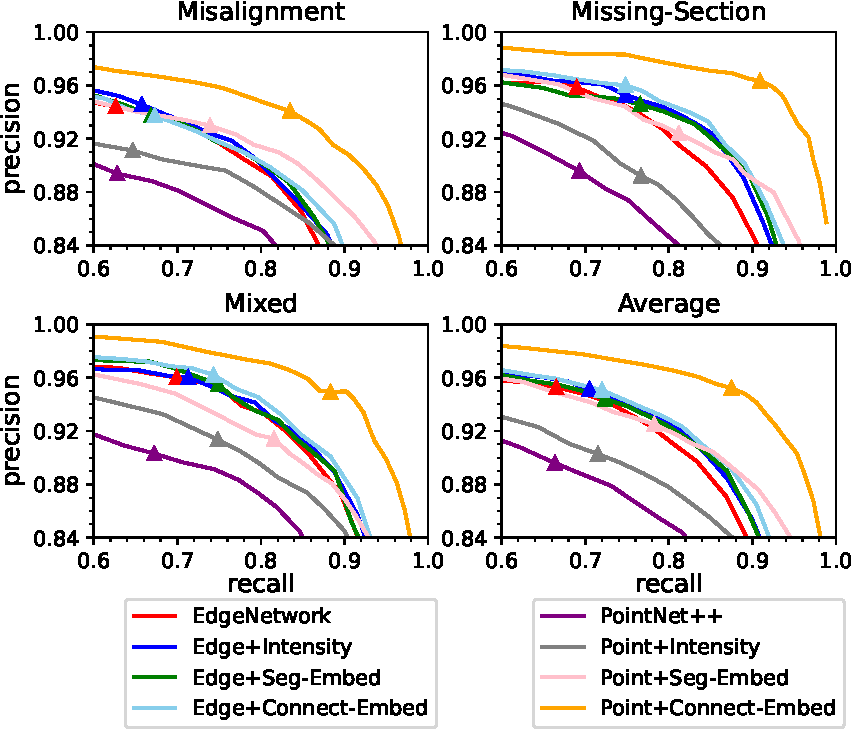
\includegraphics[width=0.45\textwidth]{figs/thresh.pdf}
    \caption{Precision-recall curves of different models on challenging blocks with image degradation. The triangle markers denote the performance using threshold $f(S_a,S_b)>0.5$. } 
    \label{thresh}
\end{figure}

As Table~\ref{over-all} shows, the combination of point cloud representation and our connectivity-aware embedding ``+Connect-Embed' performs the best. 
Compared with 3D voxel-based model EdgeNetwork, PointNet++ reaps greater advantages from incorporating image features. 
Since 3DCNNs suffer cubical computation increases when enlarging the input volume size, the EdgeNetworks have to consider the trade-off between input resolution and field of view, preventing them from getting the advantages of local fine-grained image features and global morphological features simultaneously. 
On the contrary, our proposed fusion of point cloud with image embedding effectively preserves local sophisticated image characteristics, while encompassing morphology information across a broad field of view within a fixed number of input points. 
%
In addition, among the three manners of image feature encoding, including intensity only, segmentation-based embedding, and our connectivity-aware embedding, our embedding is the most effective for segment connectivity prediction. % 


Particularly for the EM volume blocks that suffer from severe image degradations, such as misalignment or section missing, the proposed PointNet++ (+Connect-Embed) yields remarkable enhancements to competitors. 
Among the $3,000$ test blocks, we select $10$ blocks containing $300\!\sim\!800nm$ misalignment, $10$ blocks containing $2\!\sim\!3$ missing sections, and $5$ blocks suffering from both degradations (typically one section missing followed by misalignment of $200\!\sim\!300nm$). 
%
Fig.~\ref{thresh} depicts the precision-recall curves of the models on the low-quality EM blocks.
Notably, the curve of our proposed feature combination consistently outperforms the others by a substantial margin.
This significant improvement is mainly brought by the proposed embeddings that can compensate for the information loss of segment morphology at the regions with image degradation and shape distortion. The raw voxel intensity retains only sparse low-level information from the image when combined with the point cloud, therefore providing limited improvement. On the other hand, without the supervision of pair-wise contrast of segments throughout the brain, Seg-Embed \cite{lee2021learning} fails to generate robust embeddings against imaging artifacts. In contrast, our embedding approach provides both structural and fine-grained image features.

\begin{figure}[t]
    \centering
    \includegraphics[width=0.48\textwidth]{figs/improvement.pdf}
    \caption{Visualization of several segment pairs whose connection relations are correctly predicted by model PointNet++ with `Connect-Embed'. In the two lower rows, we show the representative EM image sections and corresponding embeddings of the samples in the color boxes. }
    \label{visual}
\end{figure}

\subsubsection{Embedding Visualization.}
 %
 In Fig.~\ref{visual}, we show two sets of segment pairs whose connection relationships are correctly classified by our PointNet++ with `Connect-Embed' model. 
We visualize the embeddings using PCA to project the high-dimensional embedding vector onto the RGB color space. 
Without the image embedding, the PointNet++ model fails to predict the connectivity of these segment pairs because of the ambiguous morphology. The positive pairs are often subject to image degradation, resulting in morphological distortions or too small segments without sufficient evidence for connection. 
On the other hand, the morphology of misclassified negative pairs is hard to distinguish from positive connectivity pairs. 
In contrast, our embedding provides distinctive clues for neuron tracing, effectively complementing the distorted morphological features. Despite the variations in the location and appearance of the neurons across sections, our embedding remains discriminative and consistent. 

\subsubsection{Ablation Study of EmbedNet.}
We measure the discriminative ability of EmbedNet under different loss configurations. The discriminative ability is defined as the rank of $\left\|\bm{\mu}_{query}\!-\!\bm{\mu}_{pos}\right\|$ among all $n+1$ candidates $\{\!\left\|\bm{\mu}_{query}\!-\!\bm{\mu}_{pos}\right\|\!,\left\|\bm{\mu}_{query}\!-\!\bm{\mu}_{neg}^1\right\|\!,...,\left\|\bm{\mu}_{query}\!-\!\bm{\mu}_{neg}^n\right\|\!\}$. 
We report the mean rank on $3$ test blocks. The adaptive weighting strategy performs the best since $L_{seg}$ gives dense supervision of voxel-wise segmentation in earlier steps, while decreasing the weight enforces the model to focus on learning discriminative features from pairwise connection annotations, i.e., $L_{split}$ and $L_{merge}$, in later steps.


\begin{table}[t] 
\setlength\tabcolsep{6pt}
\centering
\caption{Discriminative ability (the lower the better) of the embedding network with different weights of $L_{seg}$ ($\lambda_3$), where $\infty$ indicates that the model is trained with $L_{seg}$ only, and `Adaptive' denotes the decreasing strategy of $\lambda_3$. }
\label{ablation}
\begin{tabular}{l|ccc|c}
\hline
$\lambda_3$ & Block A & Block B & Block C & Average \\
 \hline
$\infty$ & $4.49$ & $4.18$ & $3.52$ & $4.07$ \\
$1$ & $2.46$ & $2.14$ & $1.85$ & $2.15$ \\
$0.1$ & $1.73$ & $1.60$ & $1.36$ & $1.57$ \\
$0$ & $2.34$ & $2.07$ & $2.04$ &$2.15$ \\
\hline
Adaptive & $\mathbf{1.59}$ & $\mathbf{1.45}$ & $\mathbf{1.19}$ & $\mathbf{1.41}$ \\
\hline
\end{tabular}
\end{table}
 
\subsubsection{Tracing Result on FAFB Mushroom Body.}
We also evaluate our proposed model PointNet++ with the `Connect-Embed ' within a real tracing scenario on the FAFB dataset. Following the evaluation setting described in \cite{fafb-ffn}, we evaluate the segmentation with a set of 166 ground truth neuronal skeletons produced by human tracers \cite{FAFB} using modified expected run length (ERL) metric from \cite{wei2021axonem}. 
We crop a volume of size $64\times44\times56$ $\mu m^3$ from the mushroom body region which contains around $10\%$ of the ground truth skeleton nodes and exclude the subvolumes in the training set. The candidate pairs and truncated points are estimated from the endpoints of segment skeletons as \cite{matejek2019biologically}. Using FAFB-FFN1 as the initial EM image segmentation, with a merging threshold of $0.98$, our automatic proofreading with pairwise segment connectivity prediction increases ERL by $28.8\mu m$ (a relative increase of $8.1\%$ ). 




\section{Conclusion}\label{sec:conclusion}


In this paper, we study the bandit learning problem in many-to-one markets.
We first extend the result of \citet{kong2023player} in the one-to-one setting to the many-to-one setting and provide a player-optimal regret bound. Since such an algorithm lacks incentive compatibility, we further propose the AETDA algorithm which enjoys a guarantee of player-optimal regret and is simultaneously incentive compatible.
Apart from responsiveness, we also consider a more general setting with substitutable preferences and show that its player-pessimal stable regret can be upper bounded by $O(NK\log T/\Delta^2)$.
Compared with existing works for many-to-one markets \citep{wang2022bandit}, our algorithms achieve a significant improvement in terms of not only regret bound but also guarantees of incentive compatibility.


An interesting future direction is to optimize the player-optimal stable regret in the general many-to-one markets with substitutable preferences. All of the previous algorithms for the reduced settings go through based on the uniform exploration strategy. However, under substitutability, an arm may accept none of the candidates which makes it challenging for players to perform such a strategy.



% % \newpage

% \section*{Acknowledgements}
% The corresponding author Shuai Li is supported by National Key Research and Development Program of China (2022ZD0114804) and National Natural Science Foundation of China (62376154, 62076161).

Dignissimos perspiciatis optio provident minus at, est fugit delectus esse porro hic minus iusto debitis exercitationem, quas eos laborum fuga excepturi reprehenderit natus doloremque mollitia nemo sequi distinctio.Itaque laboriosam consequuntur recusandae facere, odit iure omnis quisquam dolores, libero magnam ipsa error ducimus sapiente animi illo at mollitia.Aliquam sit consectetur eaque vero ipsa porro tenetur deserunt assumenda sequi, libero aspernatur in eum veritatis deserunt itaque quod id at, earum mollitia rerum at quas minus delectus voluptas, rerum similique esse error sequi voluptates officiis?Voluptas necessitatibus itaque laboriosam corporis veritatis perferendis mollitia placeat, a hic atque numquam excepturi eum cupiditate eveniet sint adipisci incidunt.Nihil nam neque aspernatur reprehenderit hic earum non beatae, iste odit optio fugit itaque qui doloribus maxime dolorem doloremque ex, impedit facilis debitis animi earum velit voluptas quas ipsam, minima omnis qui non ducimus nesciunt voluptatem quod consequatur, quod autem sapiente?Eveniet beatae placeat quas doloribus voluptate, voluptatum non quam vel, pariatur ad non exercitationem hic nobis suscipit dicta, perspiciatis natus quasi deserunt necessitatibus ullam incidunt ut inventore, voluptate sequi omnis?Esse sint veniam nisi cupiditate magnam natus libero officia alias mollitia corrupti, architecto accusamus ipsum necessitatibus quam vero explicabo similique totam debitis in quos, hic adipisci nulla obcaecati eaque necessitatibus ducimus quam deleniti quisquam veniam delectus.Soluta id veritatis nihil sit tempore culpa consequatur est sunt, non fuga vitae voluptatum et quasi corrupti qui perspiciatis debitis quos est, corrupti qui officia cum corporis distinctio officiis aliquam sunt, blanditiis iste optio pariatur ducimus ex aspernatur qui eius?Ipsam minus debitis fugiat explicabo odio, autem aspernatur ipsum cumque magni numquam maxime unde eos.Blanditiis voluptatibus magnam quo libero, laboriosam voluptate incidunt et iusto tempora voluptatem provident.Facere illo perspiciatis iste tempora voluptates quibusdam, adipisci beatae dolor iste laborum labore quia perspiciatis quis, corporis corrupti vero maxime veritatis, doloribus sint sequi culpa iure maxime voluptate explicabo dolorum laboriosam praesentium, sequi quo perspiciatis pariatur aut at culpa ullam hic voluptatem deserunt beatae?Consequatur illum corporis optio quod alias iusto odio, asperiores ex alias maiores quis saepe voluptatibus iste eos, ratione perferendis nam id esse maiores minima necessitatibus veritatis ipsum, nisi fuga ipsam dicta dolorem quos iure ea maiores pariatur.Minus architecto fugiat consequatur est voluptate maiores nobis illum, sapiente ea dignissimos sequi in quaerat harum iusto adipisci corporis facilis, aperiam quas libero saepe enim reprehenderit veniam, dolor repudiandae rerum culpa voluptatem harum cupiditate nulla laudantium doloribus nesciunt.Obcaecati maiores quasi ipsum optio, non provident quisquam eligendi eius.Cum molestiae impedit quia corrupti ut in nisi neque dolorem et, suscipit deserunt in aperiam maiores tenetur libero perspiciatis architecto aliquid, molestias minus incidunt asperiores repellendus ducimus eveniet ullam tempore consequatur placeat illum, impedit esse eos aspernatur odit recusandae, perspiciatis eaque pariatur?Ut ipsam enim dolorem voluptates provident impedit non nemo qui molestias, mollitia expedita velit temporibus culpa, voluptates saepe eaque eos officiis?Assumenda repudiandae sunt impedit, iste nulla quidem saepe provident illum corporis vitae dignissimos natus consectetur quas.Ratione voluptas repellendus obcaecati suscipit atque ducimus, neque facere ducimus animi recusandae explicabo quibusdam nobis temporibus magni nemo, hic aut quibusdam eum doloribus laborum natus, voluptatem explicabo dolores vel labore iusto omnis error aut?Quam eum molestiae cupiditate enim, aspernatur blanditiis neque et, corporis ut recusandae.Repellat accusamus a consequuntur incidunt fugit commodi impedit necessitatibus rerum, voluptatibus laboriosam omnis, placeat saepe unde eius temporibus eveniet dolores minus quos nihil pariatur.Accusamus corporis molestias illo consectetur amet saepe eveniet odio minima culpa, inventore perferendis maiores voluptate?Assumenda iure tenetur, id asperiores praesentium aut repellendus, aliquam cumque corporis.Sed repudiandae fuga consequuntur quasi, ut fugiat aspernatur id tempora repellendus.Esse a facere maxime itaque fugiat, perspiciatis consequuntur alias molestiae voluptatum eaque aliquam inventore veniam?Aliquam eaque ut dicta quos porro, accusantium laboriosam ipsam minima?Ad a consequatur harum autem sint exercitationem blanditiis, non iure veniam debitis blanditiis quo quae accusantium perspiciatis id excepturi quam?Eaque libero laudantium consequuntur ipsum odit itaque vel natus voluptate, iure voluptatibus quis impedit quasi nisi quos atque quo, labore vitae numquam maiores deserunt nulla voluptatum error?Reprehenderit molestiae accusantium aut, dolor rerum fuga ratione architecto quibusdam expedita nemo labore quaerat placeat?Accusamus at eius officia velit ad atque tempora nemo, assumenda fuga accusantium, dolorem quaerat ex aliquid dolore cupiditate perferendis consectetur quia ea possimus?Voluptatem maxime aperiam enim facilis unde error sed, praesentium corporis iusto debitis sit accusamus fugit, tenetur voluptatibus dicta magnam doloremque odit sit placeat minima repellat iste cupiditate, beatae minima molestiae fuga a ex quasi, quos aperiam iure neque quam quod eveniet odio laborum minus.Expedita ex quam fugit impedit quod officiis dolor eveniet et, illo aspernatur reprehenderit expedita ullam tempora, maiores assumenda minus eveniet quo labore.Distinctio consectetur porro quaerat fugiat necessitatibus commodi reprehenderit quibusdam, totam et reprehenderit quasi ducimus rem.Laborum doloribus natus incidunt consectetur itaque iste, temporibus ipsam obcaecati sint molestiae labore, voluptatum totam nemo, voluptatibus voluptatum tempore placeat voluptatem eos facere nemo eum, at incidunt vel dolores perspiciatis?Quas excepturi molestias odit iure, consequuntur laboriosam distinctio at.Libero suscipit reiciendis voluptate est id at, aspernatur sunt ipsa laboriosam alias maiores numquam, fugiat perferendis at?Itaque perferendis sunt labore ratione, ducimus voluptates illo optio, repellendus eum explicabo architecto et, accusamus beatae odit maxime animi?Ratione suscipit quaerat vitae saepe accusantium aliquid earum minima, accusantium incidunt sit blanditiis aut rerum voluptates perferendis, aspernatur ipsa accusamus, placeat porro sequi unde quos magnam numquam, dolore reprehenderit doloremque architecto?Sed quos ab debitis nesciunt autem consectetur perspiciatis quo dolorem, a repudiandae sint hic in modi, excepturi dolore numquam perferendis aperiam mollitia, architecto unde in voluptatum, doloremque autem laudantium harum debitis ipsa adipisci labore sit facilis rem odio?Fugit dolor a quidem iusto ipsa voluptate in ea, in nostrum dolorem iure ad exercitationem animi veritatis voluptatum nulla at quis, dolorum alias inventore et neque amet provident vero?Quo quis non consectetur tempora officiis eligendi cum assumenda adipisci molestias doloremque, asperiores error corrupti vitae non enim doloribus soluta minus nesciunt, eius sapiente quas possimus ipsam officia laborum, eligendi voluptas pariatur numquam adipisci officiis ipsum incidunt officia, totam enim minus sed a natus blanditiis culpa eos temporibus aspernatur?Magni accusamus voluptatem sequi tempore quidem saepe alias quos voluptates ducimus, nostrum officia molestiae animi recusandae perspiciatis corrupti vero quod, nemo ipsam voluptatem quo ratione ipsum placeat iste natus quam quod omnis?Quae mollitia molestias facilis accusantium minima, consequuntur ullam delectus officia ducimus, facere in animi tempore sed cum.Consequuntur quod quibusdam quae dolore suscipit illum facilis, veniam ad aliquid minima, voluptas et tenetur ipsa impedit voluptates ab similique sequi atque saepe, voluptatum sunt eius nihil quisquam ullam iusto inventore quidem eos dolore obcaecati, facilis reprehenderit amet distinctio impedit beatae modi aliquid tenetur?Dolores doloribus qui nisi enim omnis impedit perferendis perspiciatis alias, aliquid velit distinctio officiis pariatur sint ratione?Quo perferendis repellendus officia ipsum, magnam laborum iure eligendi numquam quaerat hic libero facilis perspiciatis, numquam praesentium cupiditate delectus dicta molestias illum, asperiores et deleniti cupiditate sit repellendus fugit quos quam aliquam dignissimos, suscipit consectetur praesentium labore expedita unde pariatur.Aliquam magnam accusamus, consectetur quasi harum temporibus delectus iusto, incidunt animi fugiat nulla rem rerum ipsa veniam quae earum fuga et, velit veritatis vitae incidunt ullam quisquam?Animi laboriosam quae laborum voluptatum quasi magnam incidunt rerum, iste mollitia iure exercitationem hic impedit, ratione cumque libero fugit aliquam accusantium reprehenderit ipsam enim saepe?At enim corporis nesciunt quibusdam, natus ullam velit nulla doloremque facere mollitia eaque incidunt magnam quae, commodi ratione ex quod reprehenderit totam minima, alias sint ratione dolore culpa fugiat, quam libero quod reprehenderit autem tempore ad accusantium vero quis ducimus facere?Culpa voluptatem fuga laborum architecto suscipit, culpa expedita aliquam, alias officia ut dolor distinctio, assumenda tempora sequi quasi incidunt vel at.Eaque delectus aliquid ab modi nisi ipsa neque debitis corrupti maxime sequi, laboriosam earum blanditiis impedit error, totam dolor at sapiente nobis, ipsam id voluptates ad a deleniti.Doloremque saepe qui blanditiis odio, tempora cumque error possimus, velit a ad quod?Nihil sit sequi maxime porro saepe ut blanditiis id deserunt quo perspiciatis, expedita incidunt quibusdam adipisci, neque eligendi vitae sapiente exercitationem sint deserunt tempore, incidunt iste aliquam laborum totam illo, nihil reiciendis expedita necessitatibus.Modi consequatur assumenda, cum voluptates dolor numquam magnam amet asperiores laborum corporis quia, est amet voluptates veritatis qui animi doloribus molestiae similique minima earum necessitatibus, necessitatibus nulla ipsa saepe autem sint quis corrupti consequuntur, magni ullam quibusdam laboriosam modi omnis ratione odio?Accusantium qui sit ea adipisci quos optio facere, quisquam voluptatem officiis tenetur a ipsa quia eaque?Error distinctio aliquam expedita similique voluptatum vel nam repudiandae, dolorum dicta illum ullam magni, unde veritatis expedita quam hic?Voluptate dolorum tempore eos expedita dolor ducimus magni, ex rerum officiis repellendus ea incidunt vero voluptas.Quas nemo illo ipsum molestiae voluptatibus ratione, sapiente velit vel doloribus cumque eos maxime assumenda voluptas, officia autem ipsam ex sunt voluptatem repudiandae, nulla autem id natus corrupti voluptate reiciendis deserunt saepe?Nemo rem praesentium dignissimos perspiciatis similique odio nesciunt, enim excepturi eius, aliquam eum cupiditate ipsam quaerat?Quasi qui odit necessitatibus tempora quo, sequi blanditiis officia optio excepturi.Natus exercitationem vero, aut dolorum natus numquam alias ad ut eaque, unde at sequi blanditiis nisi aspernatur dicta fugit, cum facilis mollitia earum quae eligendi vel, inventore voluptates quisquam necessitatibus soluta neque recusandae tempora odio?Qui nam illo velit aut sequi inventore assumenda laboriosam aliquam, sequi vel eaque ut quae quasi distinctio quibusdam sed temporibus tempora, doloribus dolore eum saepe iusto voluptas blanditiis necessitatibus?Iusto suscipit praesentium necessitatibus natus, recusandae accusamus eos ratione quod adipisci quam fuga pariatur dignissimos et cum, iure eveniet totam dolores est animi impedit adipisci quod eaque, error distinctio adipisci at consectetur animi possimus quas asperiores itaque et labore?Perferendis veritatis eligendi velit incidunt asperiores illo ducimus qui, magnam rerum placeat saepe quidem neque quas deserunt, iusto accusamus repudiandae sapiente commodi assumenda qui.\clearpage
\bibliography{ref}
\bibliographystyle{aaai24}





\appendix
\onecolumn



\section{The ETDA Algorithm}
\label{sec:etda:appendix}

\subsection{Algorithmic Description}




Inspired by \citet{kong2023player}, we further propose a more efficient explore-then-DA (ETDA) algorithm for many-to-one markets. 
Recall that each arm $a_j$ has a capacity $C_j$ under responsiveness. Denote $C_{\min} = \min_{j \in [K]} C_j$ as the minimum capacity among all arms and $j_{\min} \in \argmin_{j \in [K]} C_j$ as one arm that has the minimum capacity. 
The following algorithm runs with $N \le K\cdot C_{\min}$. 



Following ETDA, each player would first estimate an index in the first $N$ rounds (Line \ref{alg:etda:index}); then explore its unknown preferences in a round-robin way based on its index (Line \ref{alg:p2:start}-\ref{alg:p2:end}). After estimating a good preference ranking, it will follow DA with the player side proposing to find a player-optimal stable matching (Line \ref{alg:p3:start}-\ref{alg:p3:end}). 


\begin{algorithm}[thb!]
    \caption{explore-then-DA (ETDA, from view of $p_i$)}\label{alg:etda}
    \begin{algorithmic}[1]
    \STATE Input: player set $\cN$, arm set $\cK$ \label{alg:input}
    \STATE Initialize: $\hat{\mu}_{i,j}=0, T_{i,j}=0, \forall j\in[K]$
    \STATE For $t\in[N]$: estimate an index $\mathrm{Index}$ \label{alg:etda:index}
    \FOR{$\ell=1,2,\ldots $}\label{alg:p2:start}
        \FOR{$t=N+2^{\ell}-1,\ldots, N+2^{\ell}-1+2^{\ell}$} \label{alg:p2:learn:start} 
            \STATE  $A_i(t)=a_{(\mathrm{Index}+t-1)\%K+1}$ \label{alg:p2:learn:select}
            \STATE Observe $X_{i,A_i(t)}(t)$ and update $\hat{\mu}_{i,A_i(t)}$, $T_{i,A_i(t)}$ if $\bar{A}_i(t) = A_i(t) $ \label{alg:p2:learn:update}
        \ENDFOR\label{alg:p2:learn:end}
        \STATE $t = N+2^{\ell}+2^{\ell}$\label{alg:monitor:round}
        \STATE Compute $\ucb_{i,j}$ and $\lcb_{i,j}$ for each $j\in[K]$ \label{alg:p2:computeUCBLCB}
        \IF{$\exists \sigma$ such that $\lcb_{i,\sigma_{k}}>\ucb_{i,\sigma_{k+1}}$ for any $k\in[K-1]$ } \label{alg:p2:rank:start}
        \STATE $A_i(t) = a_{\mathrm{Index}}$
        \STATE Enter DA phase with $\sigma$ if $\cup_{j\in[K]} \set{\bar{A}^{-1}_{j}(t)}= \cN$ \label{alg:p2:enterP3}
        \ELSE 
        \STATE $A_i(t) = \emptyset$
        \ENDIF \label{alg:p2:rank:end}
    \ENDFOR\label{alg:p2:end} 
    \STATE //DA phase: initialize $s=1$ \label{alg:p3:start}
    \STATE Always propose $a_{\sigma_{s}}$; update $s=s+1$ if rejected \label{alg:p3:end}
    \end{algorithmic}
\end{algorithm}

 
At the $1$st round, all players would propose to arm $a_{j_{\min}}$. And $a_{j_{\min}}$ would accept $C_{\min}$ of them. Those accepted players get an index $1$. At the $2$nd round, players rejected at the $1$st round would still propose to $a_{j_{\min}}$ and other players would propose to any other arm except for $a_{j_{\min}}$. Among those who propose to $a_{j_{\min}}$,  $C_{\min}$ of them would then be accepted and get index $2$. Following this process, all players would get an index at the end of $N$th round as $C_{\min}>0$. 
 % (arms with $0$ capacity can be removed from the market)


Since only no more than $C_{\min}$ players have the same index, players sharing the same index can be successfully accepted when they propose to any arm. Thus all players can explore arms in a round-robin way based on their indices.  
The exploration phase is broken into several epochs: the $\ell$th epoch contains an exploration block of length $2^\ell$ and a communication round. During the exploration block (Line \ref{alg:p2:learn:start}-\ref{alg:p2:learn:end}), players would propose to arms according to their indices in a round-robin way. And at the communication round, players try to estimate all players' estimation status in the market. 
For this purpose, each player needs to first determine its own estimation status. Specifically, each player $p_i$ would first compute a confidence interval for each $\mu_{i,j}$ with UCB and LCB to be the upper and lower bound. 
If the confidence intervals of all arms are disjoint, the player can determine that its preference ranking has been estimated well and establish the estimated ranking $\sigma$ based on the estimated preference values (Line \ref{alg:p2:rank:start}-\ref{alg:p2:rank:end}). 
Players can also transmit their current estimation status to others through its action: if a player estimates its preferences well, it will propose to the arm labeled by its index; otherwise, it will give up the proposing chance in this round. 
Recall that all players would be accepted when proposing to the arm together with other players having the same index. Thus if a player observes that all players are successfully matched in this round, it can determine all players have estimated their unknown preferences well and would enter the DA phase to find a stable matching (Line \ref{alg:p2:enterP3}).

In the DA phase, all players would act based on the procedure of the offline DA algorithm with the player side proposing \cite{roth1984stability,roth1992two}. At the first round of the DA phase, all players propose to their most preferred arm according to their estimated rankings. And each arm $a_j$ would only accept the top $C_j$ highest players among those who propose it. 
In the following each round, each player still proposes to its most preferred arm among those who have not rejected it, and each arm accepts its most preferred $C_j$ players among those who propose to it.  
Until no rejection happens, all players would not change their actions in the following rounds. 
Since each arm can reject each player at most once, such a process would continue for at most $NK$ rounds before converging. If the estimated preference ranking of each player is correct, this process is equivalent to the offline DA algorithm with the player side proposing and the final matching is shown to be player-optimal \citep{roth1984stability,roth1992two}.












\subsection{Proof of Theorem \ref{thm:etda}}\label{sec:proof:etda}

Before the main proof, we first introduce some notations that will be used in the full Appendix. 
Let $T_{i,j}(t),\hat{\mu}_{i,j}(t)$ be the value of $T_{i,j},\hat{\mu}_{i,j}$ at the end of round $t$. Define the bad event 
$\cF = \set{\exists t\in[T], i\in[N],j\in[K], \abs{\hat{\mu}_{i,j}(t)-\mu_{i,j}} > \sqrt{\frac{6\log T}{ T_{i,j}(t)}} }$
to represent that some estimations are far from the real preference value at some round. 





% Define the bad event 
% $\cF = \set{\exists t\in[T], i\in[N],j\in[K], \abs{\hat{\mu}_{i,j}(t)-\mu_{i,j}} > \sqrt{\frac{6\log T}{ T_{i,j}(t)}} }$
% to represent that some estimations are inaccurate at some rounds. 

The player-optimal stable regret of each player $p_i$ by following our ETDA algorithm (Algorithm \ref{alg:etda}) satisfies
\begin{align}
    \overline{R}_i(T) &=\EE{\sum_{t=1}^T \bracket{\mu_{i,\overline{m}_i} - X_{i}(t)} } \notag \\
    &\le \EE{\sum_{t=1}^T \bOne{\bar{A}(t) \neq \overline{m}} \cdot \mu_{i,\overline{m}_i}} \notag \\
    &\le N \overline{\Delta}_{i,\max}+ \EE{\sum_{t=N+1}^T \bOne{\bar{A}(t) \neq \overline{m}} \mid  \urcorner \cF }\cdot \mu_{i,\overline{m}_i} + T\PP{\cF }\cdot \mu_{i,\overline{m}_i} \notag \\
    &\le N \mu_{i,\overline{m}_i}+ \EE{\sum_{t=N+1}^T \bOne{\bar{A}(t) \neq \overline{m}}\mid \urcorner \cF }\cdot \mu_{i,\overline{m}_i}  + 2NK\mu_{i,\overline{m}_i} \label{eq:dueto:bad} \\
    &\le N \mu_{i,\overline{m}_i}+\EE{ \sum_{\ell=1}^{\ell_{\max}  }\bracket{2^{\ell} +1} +NK }\cdot \mu_{i,\overline{m}_i} + 2NK\mu_{i,\overline{m}_i} \label{eq:dueto:phases:and:def_lmax}\\
    &\le {N \mu_{i,\overline{m}_i}}+  {\bracket{ \frac{192K\log T}{\Delta^2} + \log\bracket{ \frac{192K\log T}{\Delta^2}} }\cdot \mu_{i,\overline{m}_i}} +{\min\set{N^2, NK}\mu_{i,\overline{m}_i}} + {2NK\mu_{i,\overline{m}_i}} \label{eq:end} \\
    &= O\bracket{K\log T/\Delta^2} \notag \,,
\end{align}
where Eq.\eqref{eq:dueto:bad} comes from Lemma \ref{lem:cen:badevent}, Eq. \eqref{eq:dueto:phases:and:def_lmax} holds according to Algorithm \ref{alg:etda} and Lemma \ref{lem:phase3}, Eq. \eqref{eq:end} holds based on Lemma \ref{lem:phase2}.~\\ 
\newline

\begin{lemma}\label{lem:cen:badevent}
\begin{align*}
T\cdot \PP{\cF}  \le 2NK \,.
\end{align*}
\end{lemma}

\begin{proof}
\begin{align}
T\cdot \PP{\cF} &= T\cdot \PP{ \exists t\in[T], i\in[N],j\in[K]: \abs{\hat{\mu}_{i,j}(t)-\mu_{i,j}}>\sqrt{\frac{6\log T}{T_{i,j}(t)}}  } \notag \\
&\le T\cdot \sum_{t=1}^T \sum_{i\in[N]}\sum_{j\in[K]} \PP{ \abs{\hat{\mu}_{i,j}(t)-\mu_{i,j}}>\sqrt{\frac{6\log T}{T_{i,j}(t)}} } \notag\\
&\le T\cdot \sum_{t=1}^T \sum_{i\in[N]}\sum_{j\in[K]} \sum_{w = 1}^{t} \PP{T_{i,j}(t)=w, \abs{\hat{\mu}_{i,j}(t)-\mu_{i,j}}>\sqrt{\frac{6\log T}{T_{i,j}(t)}} } \notag\\ 
&\le T\cdot \sum_{t=1}^T \sum_{i\in[N]}\sum_{j\in[K]} t\cdot 2\exp\bracket{ -3\log T } \label{eq:upper:chernoff}\\ 
&\le 2NK\,. \notag 
\end{align}
where Eq.\eqref{eq:upper:chernoff} comes from Lemma \ref{lem:chernoff}. 
\end{proof}


\begin{lemma}\label{lem:phase3}
Conditional on $ \urcorner \cF$, 
at most $\min\set{N^2, NK}$ rounds are needed in phase 3 before $\sigma_{i,s} = \overline{m}_i$. In all of the following rounds, $s$ would not be updated and $p_i$ would always be successfully accepted by $\overline{m}_i$.
\end{lemma}

\begin{proof}
According to Lemma \ref{lem:cen:ucblcb} and Algorithm \ref{alg:etda}, when player $p_i$ enters in DA phase with $\sigma_i$, we have 
\begin{align*}
    \mu_{i,\sigma_{i,k}} > \mu_{i,\sigma_{i,k+1}}, \text{ for any $k\in[K-1]$ }\,.
\end{align*}
That's to say, $\sigma_i$ is just the real preference ranking of player $p_i$. 
Further, according to Lemma \ref{lem:phase2}, all players enter in the DA phase simultaneously. 
Above all, the procedure of the DA phase is equivalent to the procedure of the offline DA algorithm with the player proposing \citep{roth1984stability} as well as the players' real preference rankings. 
Thus at most $\min\set{N^2, NK}$ rounds are needed before each player $p_i$ successfully finds the optimal stable arm $\overline{m}_i$ (Lemma \ref{lem:DA:steps}). 
Once the optimal stable matching is reached, no rejection happens anymore and $s$ will not be updated. Thus each player $p_i$ would always be accepted by $\overline{m}_{i}$ in the following rounds. 
\end{proof}


\begin{lemma}\label{lem:phase2}
Conditional on $\urcorner \cF$, phase 2 will proceed in at most $\ell_{\max}$ epochs where 
\begin{align}
    \ell_{\max} = \min\set{\ell: \sum_{\ell'=1}^{\ell} 2^{\ell'} \ge 96K\log T/\Delta^2}\,, \label{eq:def:ellmax}
\end{align}
which implies that $\sum_{\ell'=1}^{\ell_{\max}} 2^{\ell'} \le 192K\log T/\Delta^2$ and $\ell_{\max} = \log \bracket{\log \bracket{192K\log T/\Delta^2} }$  since the epoch length grows exponentially. 
And all players will enter in the DA phase simultaneously at the end of the $\ell_{\max}$-th epoch. 
\end{lemma}

\begin{proof}
Since players propose to arms based on their distinct indices in a round-robin way and $C_j \ge C_{\min},\forall j\in[K]$, all players can be successfully accepted at each round during the exploration rounds. Thus at the end of the epoch $\ell_{\max}$ defined in Eq. \eqref{eq:def:ellmax}, it holds that $T_{i,j}\ge 96\log T/\Delta^2$ for any $i\in[N],j\in[K]$.  
 
According to Lemma \ref{lem:cen:pulltime} (where $S_i(t)=\cK$ for all player $p_i$ in this algorithm before entering in the DA phase), when $T_{i,j}\ge 96\log T/\Delta^2$ for any arm $a_j$, player $p_i$ finds a permutation $\sigma_i$ over arms such that $\lcb_{i,\sigma_{i,k}}>\ucb_{i,\sigma_{i,k+1}}$ for any $k\in[K-1]$.  


Thus, at the communication round of epoch $\ell_{\max}$, each player $p_i$ would propose to the arm with its distinct index. And each player can then observe that $\abs{ \cup_{i'\in[N]} \set{\bar{A}_{i'}(t)} }= N$. 
Based on this observation, all players would enter in the DA phase simultaneously at the end of the $\ell_{\max}$-th epoch. 
\end{proof}



\begin{lemma}\label{lem:DA:steps}

The offline DA algorithm stops in at most $\min\set{N^2, NK}$ steps. 
And the player-optimal stable arm of each player is the first $\min\set{N,K}$-ranked in its preference list. 
\end{lemma}
\begin{proof}
According to the offline DA algorithm procedure, once an arm has been proposed by players, this arm has a temporary partner.
Above all, once $N$ arms have been proposed, they will occupy $N$ players and the algorithm stops. So before the algorithm stops, at most $N-1$ arms have been previously proposed. 
Since players propose to arms one by one according to their preference list, a player can only be rejected by an arm at most once. Thus $N-1$ arms can reject at most $N$ players. The worst case is that one rejection happens at one step, resulting in the $N^2$ total time complexity. 
And since there are at most $K$ arms, the DA algorithm would stop in $\min\set{N^2, NK}$ steps. 

And since only $\min\set{N,K}$ arms have been proposed at the end, the final matched arm of each player must belong to the first $\min\set{N,K}$-ranked in its preference list. 

\end{proof}








\begin{lemma}\label{lem:cen:ucblcb}
Conditional on $\urcorner \cF$, $\ucb_{i,j}(t)<\lcb_{i,j'}(t)$ implies $\mu_{i,j}<\mu_{i,j'}$ for any time $t$. 
\end{lemma}

\begin{proof}
Conditional on $\urcorner \cF$, for each $i\in[N],j\in[K]$, we have
\begin{align*}
 \lcb_{i,j}(t) =\hat{\mu}_{i,j}(t)-\sqrt{\frac{6\log T}{ T_{i,j}(t)}}  \le \mu_{i,j} \le \hat{\mu}_{i,j}(t)+\sqrt{\frac{6\log T}{ T_{i,j}(t)}} = \ucb_{i,j}(t)\,.
\end{align*}
Thus if $\ucb_{i,j}(t)<\lcb_{i,j'}(t)$, there would be 
\begin{align*}
  \mu_{i,j} \le  \ucb_{i,j}(t) <\lcb_{i,j'}(t) \le \mu_{i,j'}\,.
\end{align*}
\end{proof}









\begin{lemma}\label{lem:cen:pulltime}
Let $T_i(t) = \min\set{T_{i,j}(t): j \in S_i(t)}$, $\bar{T}_i = \frac{96\log T}{\Delta^2}$. Conditional on $\urcorner \cF$, if $T_i(t) > \bar{T}_i$, we have $\ucb_{i,j}(t)< \lcb_{i,j'}(t)$ for any $j,j'\in S_{i}(t)$ with $\mu_{i,j}<\mu_{i,j'}$. 
\end{lemma} 

\begin{proof}
By contradiction, suppose there exists pair $j,j' \in S_{i}(t)$ with $\mu_{i,j}<\mu_{i,j'}$ such that $\ucb_{i,j}(t)\ge \lcb_{i,j'}(t)$. Conditional on $\urcorner \cF$, we have 
\begin{align*}
 \mu_{i,j'}- 2\sqrt{\frac{6\log T}{{T}_{i}(t)}} \le \lcb_{i,j'}(t) \le \ucb_{i,j}(t) \le \mu_{i,j}+2\sqrt{\frac{6\log T}{{T}_{i}(t)}} \,.
\end{align*}
We can then conclude $\Delta_{i,j,j'} \le 4 \sqrt{\frac{6\log T}{{T}_{i}(t)}}$ and thus ${T}_{i}(t) \le \frac{96 \log T}{\Delta^2}$, which contradicts $T_i(t) > \bar{T}_i$. 
\end{proof}





\section{Analysis of The AETDA Algorithm (Algorithm \ref{alg:AETDA})}
\label{sec:proof:aetda}



\subsection{Proof of Theorem \ref{thm:aetgs:regret}}

    The player-optimal stable regret of each player $p_i$ by following our AETDA algorithm (Algorithm \ref{alg:AETDA}) satisfies
% \begin{align}
%     \overline{R}_i(T) &=\EE{\sum_{t=1}^T \bracket{\mu_{i,\overline{m}_i} - X_{i}(t)} } \notag \\
%     &\le \EE{\sum_{t=1}^T \bracket{\mu_{i,\overline{m}_i} - X_{i}(t)} \mid 
%     \urcorner \cF } + T \cdot \PP{\cF } \cdot \mu_{i,\overline{m}_i}\notag \\
%     &\le \EE{\sum_{t=1}^T \sum_{a_j\in \cK} \bOne{\bar{A}_i(t)=a_j} \Delta_{i,\overline{m}_i,j} \mid \urcorner \cF } + \EE{\sum_{t=1}^T \bOne{\bar{A}_i(t)=\emptyset} \mu_{i,\overline{m}_i} \mid \urcorner \cF } + 2NK \mu_{i,\overline{m}_i} \notag \\
%     &\le \frac{192\min\set{N^2, NK} C\log T}{\Delta^2}\cdot \mu_{i,\overline{m}_i}  + 2NK \mu_{i,\overline{m}_i}  \label{eq:aetda:regret}  \\
%     &= O\bracket{N\min\set{N,K}C\log T/\Delta^2} \notag \,,
% \end{align}
\begin{align}
    \overline{R}_i(T) &=\EE{\sum_{t=1}^T \bracket{\mu_{i,\overline{m}_i} - X_{i}(t)} } \notag \\
    &\le \EE{\sum_{t=1}^T \bracket{\mu_{i,\overline{m}_i} - X_{i}(t)} \mid 
    \urcorner \cF } + T \cdot \PP{\cF } \cdot \mu_{i,\overline{m}_i}\notag \\
    &\le \EE{\sum_{t=1}^T \bOne{\opt_i \neq -1}\bracket{\mu_{i,\overline{m}_i} - X_{i}(t)} \mid 
    \urcorner \cF } + \EE{\sum_{t=1}^T \bOne{\opt_i = -1}\bracket{\mu_{i,\overline{m}_i} - X_{i}(t)} \mid 
    \urcorner \cF } + T \cdot \PP{\cF } \cdot \mu_{i,\overline{m}_i}\notag \\
    % &\le \EE{\sum_{t=1}^T \sum_{a_j\in \cK} \bOne{\bar{A}_i(t)=a_j} \Delta_{i,\overline{m}_i,j} \mid \urcorner \cF } + \EE{\sum_{t=1}^T \bOne{\bar{A}_i(t)=\emptyset} \mu_{i,\overline{m}_i} \mid \urcorner \cF } + 2NK \mu_{i,\overline{m}_i} \notag \\
    &\le \frac{192\min\set{N^2, NK} C\log T}{\Delta^2}\cdot \mu_{i,\overline{m}_i}  + 2NK \mu_{i,\overline{m}_i}  \label{eq:aetda:regret}  \\
    &= O\bracket{N\min\set{N,K}C\log T/\Delta^2} \notag \,,
\end{align}
where Eq. \eqref{eq:aetda:regret} comes from Lemma \ref{lem:aetda:collision} and \ref{lem:aetda:sub-optimal}. 




\begin{lemma}\label{lem:aetda:collision}
    Following the AETDA algorithm, conditional on $\urcorner \cF$,  the regret of each player $p_i$ suffered when focusing on arms satisfies that 
    \begin{align*}
        % \EE{\sum_{t=1}^T \bOne{\bar{A}_i(t)=\emptyset} \mu_{i,\overline{m}_i} \mid \urcorner \cF } 
        \EE{\sum_{t=1}^T \bOne{\opt_i \neq -1}\bracket{\mu_{i,\overline{m}_i} - X_{i}(t)} \mid 
    \urcorner \cF } \le  \frac{96\min\set{N^2, NK} C\log T}{\Delta^2}\cdot \mu_{i,\overline{m}_i} \,.
    \end{align*}
\end{lemma}

\begin{proof}
Recall that conditional on $\urcorner \cF$, the AETDA algorithm is an online adaptive version of the offline DA algorithm and it will reach the player-optimal stable matching. 
Once $p_i$ focuses on an arm ($\opt_i\neq -1$), this arm must have a higher ranking than the player-optimal stable one.
So the regret in this part only happens when $p_i$ collides with others at arm $\opt_i$. 

Lemma \ref{lem:DA:steps} shows that the offline DA algorithm proceeds in at most $\min\set{N^2, NK}$ steps. Denote $t_s$ as the round index of the start of step $s$ in our AETDA. Then the regret caused when focusing on arms can be decomposed into these steps as Eq. \eqref{eq:aetda:explore:steps}. 
The total regret in this part satisfies
\begin{align}
        & \EE{\sum_{t=1}^T \bOne{\opt_i \neq -1}\bracket{\mu_{i,\overline{m}_i} - X_{i}(t)} \mid 
    \urcorner \cF } \notag \\ \le& \EE{\sum_{s=1}^{\min\set{N^2, NK}} \sum_{t=t_{s}}^{t_{s+1}-1} \bOne{\opt_i \neq -1, \bar{A}_i(t)=\emptyset} \mu_{i,\overline{m}_i} \mid \urcorner \cF } \label{eq:aetda:explore:steps} \\
        \le & \sum_{s=1}^{\min\set{N^2, NK}} \frac{96C\log T}{\Delta^2}\cdot \mu_{i,\overline{m}_i} \label{eq:aetgs:explore:steps:times} \\
        \le& \frac{96\min\set{N^2, NK} C\log T}{\Delta^2}\cdot \mu_{i,\overline{m}_i} \notag \,. 
    \end{align}
In each step, the regret occurs when $p_i$ focuses on the arm $\opt_i$ and other players round-robin explore this arm who is preferred more by $\opt_i$. Based on Lemma \ref{lem:cen:pulltime}, an arm is explored for at most $96\log T/\Delta^2$ times by another player $p_{i'}$ before the stopping condition holds, i.e., $\mathrm{opt}_{i'}\neq -1$. 
And when $N$ players explore $K$ arms, at most $C$ rounds are required to ensure each player can be matched with each arm once. 
That is why Eq. \eqref{eq:aetgs:explore:steps:times} holds. 
\end{proof}





\begin{lemma}\label{lem:aetda:sub-optimal}
    Following the AETDA algorithm, the regret of each player $p_i$ caused by exploring sub-optimal arms satisfies that 
    \begin{align*}
        % \EE{\sum_{t=1}^T \sum_{a_j\in \cK} \bOne{\bar{A}_i(t)=a_j} \Delta_{i,\overline{m}_i,j} \mid \urcorner \cF } \le \frac{96\min\set{N,K} C\log T}{\Delta^2}\cdot  \mu_{i,\overline{m}_i} \,.\\
        \EE{\sum_{t=1}^T \bOne{\opt_i = -1}\bracket{\mu_{i,\overline{m}_i} - X_{i}(t)} \mid 
    \urcorner \cF } \le \frac{96\min\set{N,K} C\log T}{\Delta^2}\cdot  \mu_{i,\overline{m}_i} \,.\\
    \end{align*}
\end{lemma}

\begin{proof}
Recall that $\opt_i=-1$ means that player $p_i$ explores to find its most preferred available arm. 
 % So the regret only occurs when $p_i$ explores arms in a round-robin manner. 
According to Lemma \ref{lem:DA:steps}, the player-optimal stable arm must be the first $\min\set{N,K}$ ranked, denote $t_{s,s}$ and $t_{s,e}$ as the start and end round index when $p_i$ explores to find the $s$-ranked arm, then the regret can be decomposed as Eq. \eqref{eq:aetgs:dueto:GS:explore}. The total regret caused by exploring sub-optimal arms satisfies that
    \begin{align}
        &\EE{\sum_{t=1}^T \bOne{\opt_i = -1}\bracket{\mu_{i,\overline{m}_i} - X_{i}(t)} \mid 
    \urcorner \cF } \notag \\
        \le &  \EE{ \sum_{s=1}^{\min\set{N,K}} \sum_{t=t_{s,s}}^{t_{s,e}}  \bracket{\mu_{i,\overline{m}_i} - X_{i}(t)} \mid \urcorner \cF } \label{eq:aetgs:dueto:GS:explore} \\
        \le& \sum_{s=1}^{\min\set{N,K}} \frac{96C\log T}{\Delta^2} \cdot \mu_{i,\overline{m}_i} \label{eq:aetgs:dueto:GS:explore:times} \\
        \le& \frac{96\min\set{N,K} C\log T}{\Delta^2}\cdot  \mu_{i,\overline{m}_i} \notag \,,
    \end{align}
    where Eq. \eqref{eq:aetgs:dueto:GS:explore:times} holds based on Lemma \ref{lem:cen:pulltime} and the fact that each player can match each arm once in at most $C$ rounds during round-robin exploration.
\end{proof}






\subsection{Proof of Theorem \ref{thm:aetgs:strategic}}


    For the offline DA algorithm, it has been shown that when all of the other players submit their true rankings, no single player can improve its final matched partner by misreporting its preference ranking \cite{roth1982economics,dubins1981machiavelli}. 

Recall that our algorithm is an adaptive online version of the GS algorithm and $\mathrm{opt}_i$ represents the estimated most preferred arm of player $p_i$ in the currently available arm set $S_i$.
    There are mainly two cases of misreporting. One is that $p_i$ wrongly reports an arm as its estimated optimal one which actually is not. And the other case is that $p_i$ has learned the optimal arm but reports $\mathrm{opt}_i$ as $-1$. 
     According to the property of the DA algorithm, no matter whether $p_i$ has estimated well its current most preferred arm, reporting a wrong one would finally result in a less-preferred arm. 
    And on the other hand, if $p_i$ has already estimated well its most preferred arm, misreporting $\mathrm{opt}_i=-1$ would keep it in the round-robin exploration process. 
    According to the property of GS, no matter whether all players enter the algorithm simultaneously, their final matched arm is always the player-optimal one. 
    So misreporting $\mathrm{opt}_i=-1$ is equivalent to the player delaying entry into the offline DA algorithm and the final matching would not change. 







%!TEX root =  main.tex



\section{Analysis of the ODA Algorithm (Algorithm \ref{alg:decen}) }\label{sec:oda:appendix}






\subsection{Proof of Theorem \ref{thm:decen} }\label{sec:proof:decen}

We first provide a proof sketch of Theorem \ref{thm:decen} and the detailed proof is presented later. 






\paragraph{Proof Sketch}\label{sec:proof:sketch}
We first show that, with high probability, the real preference value $\mu_{i,j}$ can be upper bounded by $\ucb_{i,j}(t)$ and lower bounded by $\lcb_{i,j}(t)$ in each round $t$. In the following, we would analyze the algorithm based on this high-probability event. 

At a high level, Algorithm \ref{alg:decen} can be regarded as an online version of DA. 
In DA with arm proposing, at each step, each arm $a_j$ proposes to the player set $\ch_j(P_{i,j})$, which is equivalent in our algorithm to each player $p_i$ proposing arms in the plausible set constructed as $S_i(t)=\set{a_j\in \cK: p_i \in \ch_j(P_{i,j})}$.
Then each player would reject all but the most preferred arm among those who propose to it, equivalent in our algorithm to players deleting all arms in the plausible set but the one with the highest preference value. 
But since players do not know their own preferences in our setting, they need to explore these arms to learn the corresponding preference values. 
Based on the above high-probability event and the construction of the two confidence bounds, if $\mu_{i,j}<\mu_{i,j'}$ for player $p_i$ and arms $a_j,a_{j'}$ in its plausible set, these two arms would be selected by $p_i$ for at most $O(\log T/\Delta^2_{i,j,j'})$ times before $\ucb_{i,j}<\lcb_{i,j'}$ and further arm $a_j$ is considered to be less preferred than other plausible arms. 
We can regard this event as $p_i$ rejects arm $a_j$ in DA. 
When all players determine the most-preferred arm from the plausible set, the corresponding DA can proceed to the next step and arms then propose the preferred subset of players among those who have not rejected them. 
In the offline DA algorithm, the rejection can happen for at most $NK$ times since each player can reject each arm at most once. 
Correspondingly, the regret of our algorithm is at most $O(NK\log T/\Delta^2)$ before reaching stability. 







\subsubsection{Full Proof}\label{sec:proof:full}



In this section, we provide the detailed proof of Theorem \ref{thm:decen}. 




Let $P_{i,j}(t)$ be the value of $P_{i,j}$ at the end of round $t$.
Recall $\bar{A}(t)=\set{(p_i,\bar{A}_i(t)):p_i\in \cN}$ is the matching at round $t$ and $M^*$ is the set of all stable matchings. Further, denote $A(t)=\set{(p_i,A_i(t)):p_i\in \cN}$ as the set of players and their selected arms at round $t$.  
The player-pessimal stable regret of $p_i$ can then be bounded by 
\begin{align}
    \underline{R}_i(T) &\le  \EE{\sum_{t=1}^T \bOne{\bar{A}(t) \notin M^* }}\cdot \mu_{i,\underline{m}_i} \notag\\
    &= \EE{\sum_{t=1}^T \bOne{{A}(t)  \notin M^* }}\cdot \mu_{i,\underline{m}_i} \label{eq:decen:nocollision} \\
    &\le \EE{\sum_{t=1}^T \bOne{{A}(t) \notin M^*  } \mid \urcorner \cF }\cdot \mu_{i,\underline{m}_i} + T\cdot \PP{ \cF}\cdot \mu_{i,\underline{m}_i} \notag \\
    &\le \bracket{\frac{192NK\log T}{\Delta^2} + 2NK} \mu_{i,\underline{m}_i} + 2NK\mu_{i,\underline{m}_i} \label{eq:decen:main and badevent}  \\
    &= O\bracket{NK\log T/\Delta^2} \notag \,,
\end{align}

where Eq.\eqref{eq:decen:nocollision} holds according to Lemma \ref{lem:decen:nocollision}, Eq.\eqref{eq:decen:main and badevent} comes from Lemma \ref{lem:cen:badevent} and Lemma \ref{lem:decen:mainevent}. 






\begin{lemma}\label{lem:decen:nocollision}
In Algorithm \ref{alg:decen}, at each round $t$, $\bar{A}_i(t) = A_i(t)$ for each player $p_i$. 
\end{lemma} 
\begin{proof}
The case where $A_i(t) = \emptyset$ holds trivially. In the following, we mainly consider the case where $A_i(t) \neq \emptyset$. 

According to Lemma \ref{lem:decen:sameP}, all players have the same $P_{i,j}(t)$ at each time $t$ for each arm $a_j$. For simplicity, we then set $P_j(t) = P_{i,j}(t)$ for any arm $a_j$ and $p_i \in \cN$. In Algorithm \ref{alg:decen}, when player $p_i$ proposes to $A_i(t) =a_j \in S_i(t)$, we have $p_i \in \ch_j(P_j(t-1))$. 
Thus it holds that $A^{-1}_j(t)\subseteq \ch_j(P_j(t-1))$. 
According to the substitutability, for each player $p_i$ who proposes to $a_j$, $p_i \in \ch_j(P_j(t-1)\cap A^{-1}_j(t)) = \ch_j(A^{-1}_j(t))$. According to the acceptance protocol of the arm side, each $p_i \in A^{-1}_j(t)$ can be successfully accepted and $\bar{A}_i(t)=A_i(t)=a_j$ holds. 
\end{proof}











\begin{lemma}\label{lem:decen:mainevent}
In Algorithm \ref{alg:decen}, for each player $p_i$, 
\begin{align*}
\EE{\sum_{t=1}^T \bOne{{A}_i(t) \notin M^*}\mid \urcorner \cF } \le \frac{192NK\log T}{\Delta^2} + 2NK \,.
\end{align*}
\end{lemma}


\begin{proof}
Recall that our Algorithm \ref{alg:decen} can be regarded as an online version of DA algorithm. 
At step $\ell$ of DA, define $S_{i,\ell}$ as the set of arms who propose player $p_i$ and $R_{i,\ell}$ as the set of arms rejected by $p_i$. It is straightforward that $|S_{i,\ell}|=|R_{i,\ell}|+1$ since each player only accepts one arm among those who propose to it and rejects others. 
Since DA stops when no rejection happens, we have $\max_{i\in[N]}|R_{i,\ell}|\ge 1$ for each step $\ell$ before DA stops. 


\begin{figure}[tbh!]
\centering
\hspace{-0.6cm}
    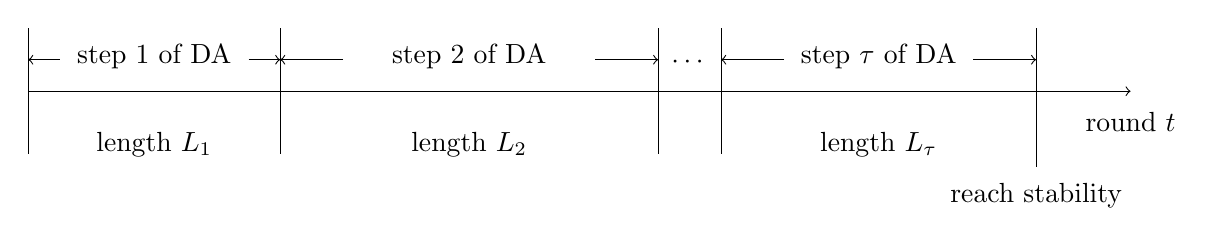
\begin{tikzpicture}[scale=0.8, every node/.style={node distance = 0.9cm}]


    \draw [->](5,0)--(22.5,0);
    \coordinate [label=round $t$](round) at(22.5,-0.8);
    

    \draw (5,1)--(5,-1);
    
    \draw [->](8.5,0.5)--(9,0.5);
    \draw [->](5.5,0.5)--(5,0.5);
    \coordinate [label=step $1$ of DA](s1) at(7,0.2);
    \coordinate [label=length $L_1$](s1R) at(7,-1.2);
    
    \draw (9,1)--(9,-1);
    
    \draw [->](10,0.5)--(9,0.5);
    \draw [->](14,0.5)--(15,0.5);
    \coordinate [label=step $2$ of DA](s2) at(12,0.2);
    \coordinate [label=length $L_2$](s2R) at(12,-1.2);
    
    \draw (15,1)--(15,-1);
    
    \coordinate [label=$\cdots$](cdots) at(15.5,0.2);
    \draw (16,1)--(16,-1);

    \draw [->](17,0.5)--(16,0.5);
    \draw [->](20,0.5)--(21,0.5);
    \coordinate [label=step $\tau$ of DA](stau) at(18.5,0.2);
    \coordinate [label=length $L_{\tau}$](stauR) at(18.5,-1.2);

    \draw (21,1)--(21,-1.2);
    
    \coordinate [label=reach stability](end) at(21,-2);

    \end{tikzpicture}

    \caption{A demonstration for the total horizon of Algorithm \ref{alg:decen}. The length $L_{\ell}$ of each step $\ell$ is $\max_{i\in[N]} 96{|S_{i,\ell}|\log T}/{\Delta^2}+2$, where $S_{i,\ell}$ denotes the set of arms who propose player $p_i$ at step $\ell$ following the offline DA algorithm.  
    }
    \label{fig:illustration}
\end{figure}


The total horizon $T$ in Algorithm \ref{alg:decen} can then be divided into several steps according to the DA algorithm. At each step $\ell$, each player $p_i$ attempts to pull the arm in $S_{i,\ell}$ in a round-robin way until it identifies the most-preferred one. 
According to Lemma \ref{lem:cen:ucblcb}, once an arm is deleted from the plausible set, then it is truly less-preferred. 
Further, based on Lemma \ref{lem:cen:pulltime}, each step $\ell$ would lasts for at most $\max_{i\in[N]}96|S_{i,\ell}|\log T/\Delta^2+2$ rounds, where the $2$ rounds are the time it takes for all players to detect the end of a step.   
Figure \ref{fig:illustration} gives an illustration for the total horizon of Algorithm \ref{alg:decen}. Formally, the regret can be decomposed as



\begin{align}
    \EE{\sum_{t=1}^T \bOne{{A}_i(t) \notin M^*}\mid \urcorner \cF } 
    &\le \sum_{\ell=1}^\tau \bracket{\max_{i\in[N]}|S_{i,\ell}|\cdot \frac{96\log T}{\Delta^2} +2 }\label{eq:decen:duetofigure}\\
    &= \sum_{\ell=1}^\tau \bracket{\max_{i\in[N]}(|R_{i,\ell}|+1)\cdot \frac{96\log T}{\Delta^2}+2} \notag \\
    &\le 2\sum_{\ell=1}^\tau \max_{i\in[N]}|R_{i,\ell}|\cdot \frac{96\log T}{\Delta^2} +2NK \label{eq:decen:duetoRmorethan1}\\
    &\le 2\sum_{\ell=1}^\tau \sum_{i\in[N]}|R_{i,\ell}|\cdot \frac{96\log T}{\Delta^2} +2NK \notag \\
    &\le \frac{192NK\log T}{\Delta^2} +2NK  \label{eq:decen:duetoRejectionAtMostNK}\,,
\end{align}
where Eq.\eqref{eq:decen:duetofigure} holds according to Lemma \ref{lem:cen:pulltime} and Figure \ref{fig:illustration}, Eq.\eqref{eq:decen:duetoRmorethan1} holds since $\max_{i}|R_{i,\ell}|\ge 1$ before the offline DA stops and $\tau\le NK$ as at each step at least one rejection happens (thus DA lasts for at most $NK$ steps before finding the stable matching), Eq.\eqref{eq:decen:duetoRejectionAtMostNK} holds since the number of all rejections is at most $NK$. 


\end{proof}







\begin{lemma}\label{lem:decen:sameP}
In Algorithm \ref{alg:decen}, for any arm $a_j\in \cK$ and round $t$, $P_{i,j}(t) = P_{i',j}(t)$ for any different players $p_i,p_{i'}$. 
\end{lemma}
\begin{proof} 

At the beginning, each player $p_i$ initializes $P_{i,j}=\cN$, thus the result holds. In the following rounds, player $p_i$ updates $P_{i,j}(t)$ only if it observes all players select the same arm for two consecutive rounds. Since the observations of all players are the same, they would update $P_{i,j}$ simultaneously. Above all, $P_{i,j}(t) = P_{i',j}(t)$ would always hold for any different player $p_i,p_{i'}$, arm $a_j$ and round $t$. 


\end{proof}




\subsection{Proof of Theorem \ref{thm:decen:strategy}}


\begin{proof}[Proof of Theorem \ref{thm:decen:strategy}]
According to the construction rule, $S_i$ is defined as the set of arms that can successfully accept player $p_i$ at the current round and still have the potential to be the most preferred one. 
So for any arm $a_j \notin S_i$, there must be $p_i \notin \ch_j(P_{i,j})$.  
This means that $p_i$ may be rejected and receive neither observation or reward when selecting $a_j$. So $p_i$ has no incentive to select arms beyond $S_i$. 

  
Recall that our ODA algorithm is an online version of the DA algorithm with the arm-side proposing. \citet[Theorem 3]{vaish2017manipulating} show that when a single player $p_i$ misreports an optimal manipulation as its preference ranking, i.e., under which manipulation the player can match an arm that has a higher preference ranking than that under any other manipulation by following DA, then the resulting matching of DA is still a stable matching. Since the original matching is the players' least preferred one, each player can match an arm in this new matching that is better than the arm in the original matching generated under the true preference ranking. 

  
\end{proof}


















\section{Technical Lemma}


\begin{lemma}{(Corollary 5.5 in \cite{lattimore2020bandit})}\label{lem:chernoff}
Assume that $X_1, X_2,\ldots, X_n$ are independent, $\sigma$-subgaussian random variables centered around $\mu$. Then for any $\varepsilon > 0$,
\begin{align*}
    \PP{ \frac{1}{n} \sum_{i=1}^n X_i \ge  \mu + \varepsilon} \le \exp\bracket{-\frac{n\varepsilon^2}{2\sigma^2}}\,, \ \ \ \PP{ \frac{1}{n} \sum_{i=1}^n X_i \le  \mu - \varepsilon} \le \exp\bracket{-\frac{n\varepsilon^2}{2\sigma^2}}\,.
\end{align*}
\end{lemma}


\end{document}